\chapter{Portfolio optimisation}
\graphicspath{{Chapter4/figures/}}
\label{cha:po}
Optimal portfolio is the ultimate goal of every investment manager; but the optimality criteria can be very different to each of them. In the infamous Markowitz's modern portfolio theory \cite{HM52}, it is assumed that investors are always interested in maximising the portfolio's return and minimising the portfolio's financial risk. For index tracker fund manager, the main objective of portfolio management is to track and replicate the exposure of a benchmark index. The lack of active management generally makes the fund less vulnerable to change of management and has the advantages of lower fees and taxes. It is the latter that the focus of the thesis lies.
 
In this chapter, we introduce the index tracking fund and summarise some causing factors of the tracking error between a fund and its benchmark index. We then present how the portfolio optimisation problem in terms of minimising the tracking error can be formulated as a stochastic control problem. We show this stochastic control problem can be turned into a path-space parameter estimation problem, in which Rao-Blackwellised SMC can be used to estimate these parameters efficiently. Lastly, we present a simple numerical example to demonstrate how to apply this technique to track a deterministic reference signal.
 
\section{Index tracking fund}
An financial index can be thought of a summary statistics of a market, typically formed as weighted average of the prices of some financial instruments. For example, FTSE 100 is an index that attempts to represent the performance of the 100 biggest companies in UK. This index is however not an investable financial product one can invest directly.
 
To allows investors to take exposure to the markets (as represented by the indices), index tracker funds are introduced. These funds generally follow very strict and transparent rules with the main objective to track their benchmark indices as close as possible. Investors of these funds therefore are only exposed to the market risks of the chosen indices, with minimal exposure to the risk associated with the investment process of the traditional active fund management.
 
\subsection{Index replication}
\label{sec:replication}
To track an index, the simplest way is to replicate the index by investing in all the components of the benchmark index. However, this can be costly and difficult to manage, considering some of the indices may have huge number of components, e.g., MSCI World Index that consists of $\approx 1600$ components from many different countries. Instead, one could partial replicate the index by sampling some of the components that are most representative. This can mean those components with larger weights, more volatiles or less correlated in returns (assuming these returns average out the gains/losses among them). This partial replication could help in reducing the transaction costs but introduce additional tracking errors to the fund.

Alternatively, the portfolio managers also have the option to enter a swap agreement with a counter-party (typically an investment bank) that provides the exact return of index in exchange for a fixed cost. Essentially, this transfers the market risk to the counter-party, at the same time, introduces the counter-party default risk. This replication technique is known synthetic replication.
 
\subsection{Causing factors of tracking error}
To evaluate the performance of an index tracking fund, different metrics have been introduced to quantify the mismatch between the performance of the fund and its benchmark index. For example, the tracking difference is the sum of absolute difference in returns between of a fund and its benchmark index. Here, we adopt the tracking error as our metric, which is defined to be the standard deviation of the absolute difference of the returns of a fund and its benchmark index defined in \cite{BJ13} as follows:
\begin{equation}
  \epsilon = \sqrt{\Var[r_p - r_b]}
\end{equation}
where $r_p$ is the return of the fund and $r_b$ is the return of the benchmark index.
 
There are many factors that can cause the tracking errors, some of which are summarised as follows:
\begin{enumerate}
\item Index rebalancing --- the benchmark index is re-weighting its constituents periodically to reflex the changes on the market based on its methodology. To track the index, the fund has to adjust its portfolio accordingly. This will incur some transaction costs. During the index rebalance period, cash drag may also  happen between the liquidation of the constituents that have weights reduced/dropped and the addition of the constituents that have weights increased/added. This cash is essentially not participating in the market and therefore it does not reflex the changes on the benchmark index.
\item Replication and sampling techniques --- funds may choose to replicate the benchmark index by selecting a subset of the constituents (often the ones with larger weights and more liquid) in an effort to minimise the transaction costs. This exclusion of the smaller, less liquid constituents may introduce another source of tracking error, especially under stressed market condition.
\item Different assumption on dividend reinvestment and taxation --- the benchmark index calculation often assumes immediate reinvestment of dividends on ex-dividend dates but the fund may only able to reinvest the dividend after receiving it. The tax treatment that is applied on the dividends may also be different.
\item Total Expense Ratio (TER) --- there is an additional expense charged to the fund on daily basis to cover the management cost.
\end{enumerate}
This list is by no mean exclusive. See \cite{BJ13} for further details.
 
\section{Methodology}
Instead of using a traditional deterministic state space models, we choose to use a \emph{stochastic} modelling approach to carry out the portfolio optimisation. In particular, we focus here the the problem in minimising the tracking error between a portfolio and its benchmark index.  Our aim is to determine what investment actions (buy or sell) a portfolio manager needs to do for each index component on a daily basis across the investment horizon to track the benchmark index well.

We adopt here a conditional Gaussian linear state space model as follows:
\begin{align}
  X_t &= A_t(U_t)X_{t-1} + B_t(U_t)W_t + F_t(U_t) \nonumber \\
  Y_t &= C_t(U_t)X_t + D_t(U_t)V_t + G_t(U_t)
\label{eq:model}
\end{align}
where $\{U_t\}_{t \geq 0}$ is a deterministic control input sequence that is used regulate the hidden states, $A_t$, $B_t$, $C_t$, $D_t$, $F_t$, $G_t$ are appropriate matrix/vector functions of $U_n$ and  $\{W_t\}_{t \geq 0}$ and  $\{V_t\}_{t \geq 0}$ are independent sequences of standard Gaussian random variables, i.e., $W_t, V_t \sim \mathcal{N}(0,I)$. The transition density and likelihood of this model are Gaussian distributions with centre lied at a point of a linear combination of the known conditional control parameters, $u_t$ of the following form:
\begin{align}
  p_t(u_t \mid u_{t-1}) &= \textrm{(any given form)} \nonumber \\
  f_t(x_t \mid x_{t-1}, u_t) &= \mathcal{N}(A_t(u_t) x_{t-1} + F_t(u_t), B_t(u_t)B_t(u_t)^T) \nonumber \\
  g_t(y_t \mid x_t, u_t)    &= \mathcal{N}(C_t(u_t) x_t + G_t(u_t), D_t(u_t)D_t(u_t)^T)
\end{align}
%This model is by no mean to compete the state of the art model in realistic portfolio optimisation, but rather to motivate further work in this direction.

Based on this model, the optimisation objective is to search for a sequence of controls $u_{1:t}$ that would result in a sequence of observations $y_{1:t}$ that tracks the reference signal $y^{ref}_{1:T}$ as close as possible. This problem is often known as stochastic regulation problem. We adopt the finite horizon multiplicative reward function proposed in \cite{NK11} here:
\begin{equation}
  J(u_{1:T},y^{ref}_{1:T}, x_0) = \E_{x_0}\left[\exp\left( -\dfrac{1}{2}\displaystyle\sum^T_{t=1}\left(\vert\vert y^{ref}_t - C_t(u_t)x_t - G_t(u_t) \vert\vert^2_{Q_t(u_t)^{-1}}  + \vert\vert u_t - u_{t-1} \vert\vert^2_{L_t}\right) \right) \right]
\end{equation}
where $Q(u_t) = D_t(u_t)D_t(u_t)^T$ and $L_t$ are assumed to known. The expectation here is taken with respect to the whole path of the Markov Chain $\{X_t\}_{t \geq 0}$ with the starting point $X_0 = x_0$,  i.e., $E_{x_0}[\phi(X_{1:t})] = \displaystyle\int \phi(X_{1:T}) \prod f_t(x_t \mid x_{t-1})~dx_{1:t}$.

The corresponding optimal open loop policy is:
\begin{equation}
  u^*_{1:T} = \arg\max_{u_{1:T}} J(u_{1:T};y^{ref}_{1:T};x_0)
\label{eq:optcontrol}
\end{equation}
with the assumption that the maximum is attainable. This reward function is closely related to the risk sensitive control discussed in \cite{WR90}, with a slight difference. This reward function used here is absence of an explicitly risk sensitive constant and it also assumes the presence of $y^{ref}_{1:T}$ as the reference target signal instead of the observable states. Nevertheless, a risk sensitivity constant could still be introduced through $D_n$ and $L_n$ if necessary.

\subsection{Problem formulation}
We assume here that the sequence of controls $\{U_t\}_{t \geq 0}$ is a Markov process with transition distribution $p(u_t \mid u_{t-1})$. The objective is to compute the marginal posterior distribution density:
\begin{equation}
 \pi_t(u_{1:t}) = p(u_{1:t} \mid y^{ref}_{1:t})
\end{equation} 
by standard marginalisation the distribution $p(x_{1:t}, u_{1:t} \mid y_{1:t})$ which in itself satisfies the following recursive equation:
\begin{align}
  p(x_{1:t}, u_{1:t} \mid y_{1:t}) = p(x_{1:t-1}, u_{1:t-1} \mid y_{1:t-1}) \frac{p(y_t \mid x_t, u_t)p(x_t, u_t \mid x_{t-1}, u_{t-1})}{p(y_t \mid y_{1:t-1})}
\end{align}
 
% This posterior density function can be derived as follows:
%\begin{align}
%p(u_{0:t} \mid y^{ref}_{0:t}) &\propto p(u_{0:t}) p(y^{ref}_{0:t} \mid u_{0:t}) \\
%&= \prod^t_{i=1} p(y^{ref} \mid y^{ref}_{0:i-1}, u_{0:i}) p(u_i \mid u_{i-1})
%\end{align}
 
%\begin{align}
%p(u_{0:t} \mid y_{0:t}) &\propto p(y_k \mid u_{0:t}, y_{0:t-1}) p(u_{0:t} \mid y_{0:t-1}) \nonumber \\
%&=  p(y_k \mid u_{0:t}, y_{0:t-1}) p(u_t \mid u_{0:t-1}, y_{0:t-1}) p(u_{0:t-1} \mid y_{0:t-1}) \nonumber \\
%&=  p(u_{0:t-1} \mid y_{0:t-1}) p(y_k \mid u_{0:t}, y_{0:t-1}) p(u_t \mid u_{t-1}, y_{0:t-1})
%\end{align}
 
One straight-forward way to approximate the recursion is directly apply SMC by consider the hidden states is a sequence of paired states $\left\{(U_t, X_t)\right\}_{t \geq 0}$. A better approach would be using the Rao-Blackwellised SMC mentioned in Section \ref{sec:msmc}, attempts to do as much computation analytically as possible, by splitting the states into the linear Gaussian states and the non-linear states. Then, the Kalman Filter can be used to model and track the linear Gaussian states and the SMC is only used to model and track the non-linear states. This marginalisation setting often yields estimates with smaller variance.

To use Rao-Blackwellised SMC on this model, we consider the following factorisation on the full posterior distribution as follows:
\begin{equation}
  p(u_{1:t}, x_{1:t} \mid y_{1:t}) = p(x_{1:t} \mid u_{1:t}, y_{1:t}) p(u_{1:t} \mid y_{1:t})
\end{equation}
Looking at the right hand side of the equation, the first term is obviously Gaussian and can therefore can be estimated optimally using Kalman Filter recursions described in Appendix \ref{sec:KF}. For the second term, we can rewrite it into the following recursion form:
\begin{align}
p(u_{1:t} \mid y_{1:t}) &\propto p(y_t \mid u_{1:t}, y_{1:t-1}) p(u_{1:t} \mid y_{1:t-1}) \nonumber \\
&=  p(y_t \mid u_{1:t}, y_{1:t-1}) p(u_t \mid u_{1:t-1}, y_{1:t-1}) p(u_{1:t-1} \mid y_{1:t-1}) \nonumber \\
&=  p(u_{1:t-1} \mid y_{1:t-1}) p(y_t \mid u_{1:t}, y_{1:t-1}) p(u_t \mid u_{1:t-1}, y_{1:t-1})
\label{eq:msmc}
\end{align}
Assuming that it is also possible to decompose the selected importance density into recursion form as follows:
\begin{equation}
        q_{1:t}(u_{1:t} \mid y_{1:t}) = q_{1:t-1}(u_{1:t-1} \mid y_{1:t-1}) q_t(u_t \mid u_{1:t-1}, y_{1:t})
\label{eq:q2}
\end{equation}
then the associated unnormalised weight of each sample can be derived in a similar fashion as given in Section \ref{sec:SIS} into the recursion form as follows:
\begin{equation}
   \tilde{w}_t  = \tilde{w}_{t-1} \dfrac{p_t(u_t \mid u_{t-1})p_t(y_t \mid u_{1:t}, y_{1:t-1})}{q_t(u_t \mid u_{1:t-1}, y_{1:t})}
   \label{eq:wsmsc}
\end{equation}
Compare to \eqref{eq:w}, the main difference here is that the weights now depends on the whole path space from time step $1$ to $t$.

\subsection{Extensions}
As discussed in Section \ref{sec:ess}, the resampling step introduces variance to the the weights, but it is necessary to avoid accumulation of estimation variance onto the weights over time. Effective sample size (ESS) can be used to measure the quality of the weight and trigger the resampling step only if necessary, e.g., 
when the ESS value at time step $t$ fall below certain threshold at time $t$, say $\frac{N}{2}$.

To add diversity in the population of particles, the Resample-Move step introduced in Section \ref{sec:rm} can also be included. This step perturbs the samples yet leave the distribution the samples represent unchanged using a MCMC kernel that is invariant in density. With this optional step in place, the whole algorithm is summarised in Algorithm \ref{algo:msmc}.

\begin{algorithm}
\caption{Rao-Blackwellised SMC to search for the optimal control parameters}\label{algo:msmc}
\begin{algorithmic}[1]
\Function{OptimalParameters}{N, T}
\State Set $t = 1$.
\State For $i \in 1, \ldots, N$, sample $u^{(i)}_1 \sim q(u^{(i)}_1 \mid y^{(i)}_1)$.
\State For $i \in 1, \ldots, N$, calculate the unnormalised importance weight:
\begin{equation*}
 \tilde{w}^{(i)}_1 = \dfrac{p(u_1^{(i)})g_1(y_1 \mid u^{(i)}_1)}{q_1(u^{(i)}_1, y_1)}
\end{equation*}
\State For $i \in 1, \ldots, N$, normalize the importance weight:
\begin{equation*}
\hat{w}^{(i)}_1 = \dfrac{\tilde{w}^{(i)}_1}{\sum^N_{j=1} \tilde{w}^{(j)}_1}
\end{equation*}
\State Set $t = t + 1$.
\While{$t \leq T$}
\State For $i \in 1, \ldots, N$, sample $u^{(i)}_t \sim q(u^{(i)}_t \mid y^{(i)}_{t-1}, u^{(i)}_{t-1})$.
\State For $i \in 1, \ldots, N$, calculate the unnormalised importance weight:
\begin{equation*}
   \tilde{w}^{(i)}_t = w^{(i)}_{t-1} \dfrac{p_t(u^{(i)}_t \mid u^{(i)}_{t-1})g_t(y_t \mid u^{(i)}_{1:t}, y_{1:t-1})}{q_t(u^{(i)}_t \mid u^{(i)}_{1:t-1}, y_{1:t})}
\end{equation*}
where
\begin{equation}
  p(y_t \mid u^{(i)}_{1:t}, y_{1:t-1}) \sim N(m_{t \mid t-1},S_t)
\end{equation}
with $m_{t \mid t-1}$ and $S_t$ are updated with Kalman Filter recursions:
\begin{align}
  \mu_{t \mid t -1} &= A_{t}(u_t)(\mu_{t-1 \mid t-1})X_{t-1} + F_t(u_t) \nonumber \\
  \Sigma_{t \mid t -1} &= A_{t}(u_t)\Sigma_{t -1 \mid t -1}A_{t}(u_t)^T +  B_t(u_t)B_t(u_t)^T \nonumber\\
  S_t &=  C_{t}(u_t)\Sigma_{t \mid t -1}C_{t}(u_t)^T +  D_t(u_t)D_t(u_t)^T \nonumber\\
  m_{t \mid t-1} &=  C_{t}(u_t)  \mu_{t \mid t-1} + G_t(u_t) \nonumber\\
  \mu_{t \mid t} &=   \mu_{t \mid t -1} +   \Sigma_{t \mid t -1} C_{t}(u_t)S_t^{-1}(y_t - m_{t \mid t-1}) \nonumber\\
  \Sigma_{t \mid t} &=  \Sigma_{t \mid t -1} -\Sigma_{t \mid t -1} C_{t}(u_t)S_t^{-1} C_{t}(u_t)\Sigma_{t \nonumber \mid t -1}
\end{align}
\State For $i \in 1, \ldots, N$, normalize the importance weight:
\begin{equation*}
\hat{w}^{(i)}_t = \dfrac{\tilde{w}^{(i)}_t}{\sum^N_{j=1} \tilde{w}^{(j)}_t}
\end{equation*}
\State \textbf{Resample:} For $i \in 1, \ldots, N$, resample $ u^{(i)}_{1:t} \sim \dfrac{\sum^N_{i=1}\hat{w}^{(i)}_t\delta_{u^{(i)}_{1:t}}}{\sum^N_{j=1} \hat{w}^{(j)}_t}$.
\State \textbf{Move:} For $i \in 1, \ldots, N$, sample $u^{(i)}_{1:t} \sim K_t(\cdot)$, where $K_t$ is $p_t$-invariant.
\EndWhile
\State Compute the MAP estimate: $\hat{u}^*_{1:t} =  \arg\max_{u_{1:t}} p(u^{(i)}_{1:t} \mid y^{ref}_{1:t})^\gamma$.
\EndFunction
\end{algorithmic}
\end{algorithm}

\subsection{MAP estimation for the control sequence}
Based on the model defined in \eqref{eq:model}, the conditional likelihood density of the model is as follows:
\begin{equation}
  g_t(y^{ref}_t \mid x_t, u_t) \propto \exp\left( -\dfrac{1}{2} \vert\vert y^{ref}_t - C_t(u_t)x_t - G_t(u_t) \vert\vert^2_{Q_t(u_t)^{-1}}\right)
\end{equation}
and the posterior distribution $p(y^{ref}_t \mid y^{ref}_{t-1}, u_{1:t})$ is as follows:
\begin{equation}
  p(y^{ref}_t \mid y^{ref}_{t-1}, u_{1:t}) \propto \exp\left( -\dfrac{1}{2} \vert\vert y^{ref}_t - m_{t \mid t-1}(u_{1:t}) \vert\vert^2_{S_t(u_{1:t})^{-1}}\right)
\end{equation}
where $m_{t \mid t-1}$ and $S_t$ are the mean and covariance matrix of the measurement at time $t$ obtained in the Kalman Filter recursions discussed in Appendix \ref{sec:KF}.

By assuming the Markov transition density for $u_t$ to be:
\begin{equation}
  p(u_{t} \mid u_{t-1}) \propto  \exp\left( -\dfrac{1}{2} \vert\vert u_t - u_{t-1} \vert\vert^2_{L_t}\right)
\label{eq:mctrans}
\end{equation}
the Maximum a Posteriori (MAP) estimate of $U_{1:T}$ is given to be:
\begin{equation}
  \tilde{u}^*_{1:t} = \arg\max_{u_{1:t}} \pi_t(u_{1:t})
\label{eq:map}
\end{equation}
which essentially specifies the model that best explains the reference $y^{ref}_{1:t}$ as the output sequence from a general set of models defined in \eqref{eq:model}.

In \cite{NK11}, it had been shown that assuming a Markov transition density for $U_t$ in \eqref{eq:mctrans}, the optimal control defined in \eqref{eq:optcontrol} and the MAP estimate defined in \eqref{eq:map} are the same. Moreover, following the monotonicity of the transformation $p(\cdot)^\gamma$, the mode of $p(\cdot)^\gamma$ is the same for all $\gamma > 0$. The main difference is that when it comes to sampling, it is easier to sample closer to the mode of the distribution when $\gamma > 1$ because the density has sharper peak and vice versa.

Putting all these together, we have the following:
\begin{equation}
  u^*_{1:t} = \tilde{u}^*_{1:t} = \arg\max_{u_{1:t}} \pi_t(u_{1:t})^\gamma,~\gamma > 0
\end{equation}
In SMC algorithm, this can be easily estimated as follows:
\begin{equation}
\hat{u}^*_{1:t} = arg\max_{u_{1:t}} \pi_t(u^{(i)}_{1:t})^\gamma = \arg\max_{u_{1:t}} p(u^{(i)}_{1:t} \mid y^{ref}_{1:t})^\gamma
\end{equation}
As long as the support of the proposal density include the support of $(u^{(i)}_{1:t} \mid y^{ref}_{1:t})$, this estimate converge asymptotically to the $\tilde{u}^*_{1:t}$ as $N \to \infty$. A better estimate can be obtained by embedding the Viterbi strategy as discussed in \cite{SG01}, but this comes with a computational cost that is quadratic in terms of the number of samples.

\section{Numerical example: Tracking an oscillating wave}
\label{sec:exp1}
We first consider here a simple linear Gaussian state space model as follows:
\begin{align}
  X_t &= X_{t-1} + W_t + U_t \nonumber \\
  Y_t &= X_t + V_t
\label{eq:refnmodel}
\end{align}
with $W_t, V_t \sim \mathcal{N}(0,I)$. This model is essential an instance of the class of model presented earlier in \eqref{eq:model}, with $A_t=B_t=C_t=D_t=I$, $F_t(U_t)=U_t$ and $G_t(U_t)=0$. The target reference is set to be an oscillating wave: $y^{ref}_t = \cos(0.2 \pi t + 0.3)$ and $L_1$ is set to $0.1$ similar to the setting used in \cite{NK11}.

This model serves two purposes here. Firstly, it is sufficient simple to verify the implementation\footnote{Strictly speaking, testing only increases confidence of the implementation correctness but does not prove no bug.}. Secondly, it serves as good benchmark problem in which we can examine the sensitivity of the algorithm to different parameter settings.

We proceed by examining the proposed SMC technique with proposal density $q_t(\cdot)$ set to be the same as the Markov transition density and all the possible combination of settings as follows:
\begin{enumerate}
\item Various time period length settings, $T$: 5, 10 and 20.
\item Various sample size settings, $N$: 100, 500, 1000, 5000 and 10000.
\item Resampling step: Always vs. Selectively (trigger condition set to be ESS $< \frac{N}{2}$).
\item Resample-Move step with MCMC (random walk proposal): Always vs. disabled.
\item Various $\gamma$ settings: Constant function of $1$, $50$, $100$, $1000$ and increasing function of time $t$, $10t$, $50t$ and $100t$.
\end{enumerate}

For each of the setting, the experiment is repeated for $30$ times. Therefore, there are in total $3 \times 5 \times 2 \times 2 \times 8 \times 30 = 14400$ runs. 

\subsection{Results and discussion}
This sections presents a summary of the experimental results from all the runs. Instead of presenting the outputs produced by all the runs, only a subset of outputs that demonstrates our findings is presented here. The complete set of implementation code and output produced can be obtained from the repository of this project at \href{https://github.com/yowtzu/mscproj}{GitHub}.

\subsubsection{Selectively resampling step with ESS}
We first evaluate the effect of selectively enabling resample step with ESS mechanism. In \emph{all} the settings, it is found that the simple runs with resample step enabled at each iteration, i.e., with ESS disabled,  always have equivalent or relative better performance in comparison to selectively resampling with ESS. Figure \ref{fig:ess} shows the result the performance obtained in terms of $\log\pi_T(\hat{u}^*_{1:t})$ of 30 independent runs of the algorithms with $T=20$ and $N=10000$ for various $\gamma$ settings. All other runs with different settings of $T$ and $N$ concur with this finding. From here onwards, we assumes ESS mechanism is disabled unless stated otherwise.

To explain this counter-intuitive result, recall that ESS is essentially a proxy to measure the quality of the weighted samples in representing the target distribution. A sample set that is well spread over the target distribution would have high ESS value and vice versa. However, the application of SMC as a maximiser here is \emph{only} concerned with the mode of the distribution. At each time step, the process of resampling the samples proportional to the weights essentially pushes the sample set towards the mode of the distribution. Selectively resampling using ESS essentially reduces the strength of this push and therefore leads to sub-optimal solution.

\begin{figure}[!thbp]
    \centering
    \begin{minipage}{.5\textwidth}
        \centering
        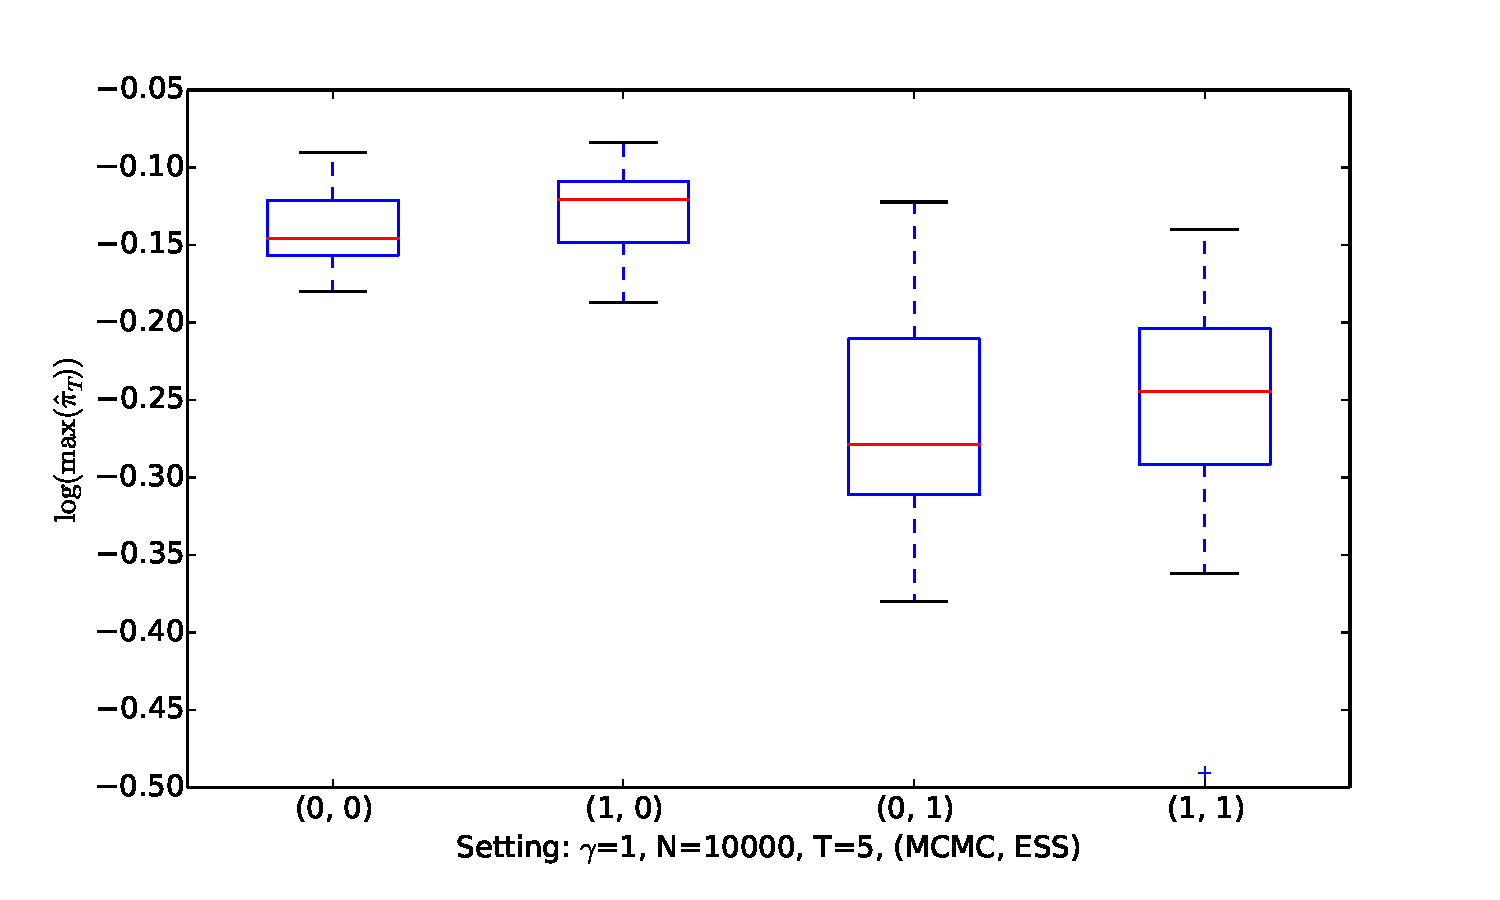
\includegraphics[width=\textwidth]{loglik_mcmc_ess/T5_gamma1_N10000.pdf}
      
        %\includegraphics[width=0.3\linewidth, height=0.15\textheight]{prob1_6_2}
        %\caption{$dt=0.1$}
        %\label{fig:prob1_6_2}
    \end{minipage}%
    \begin{minipage}{0.5\textwidth}
        \centering
        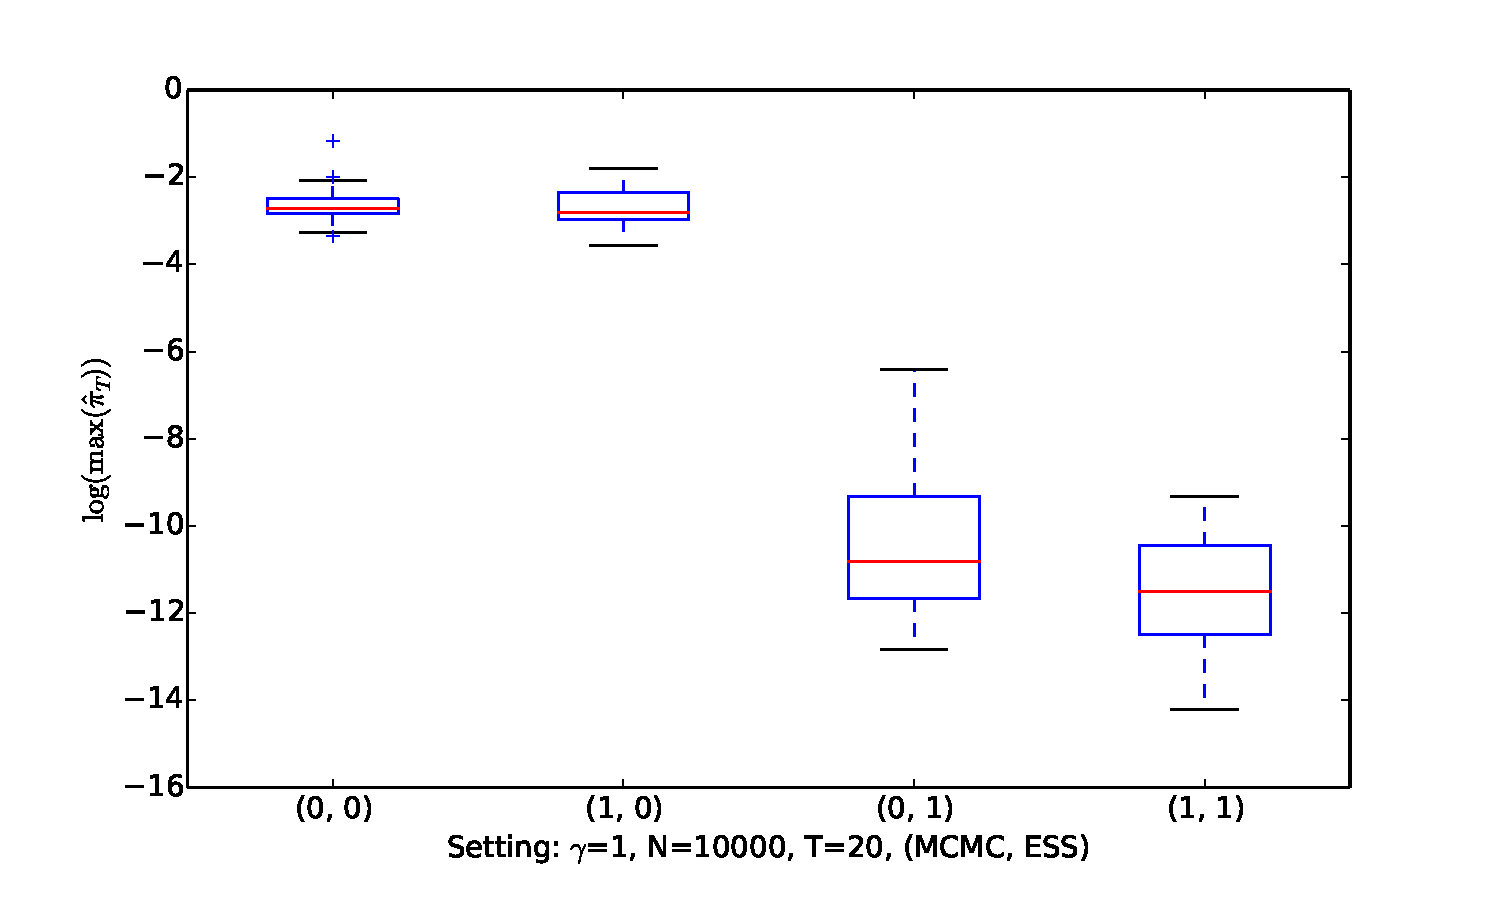
\includegraphics[width=\textwidth]{loglik_mcmc_ess/T20_gamma1_N10000.pdf}
      
    \end{minipage}
    \begin{minipage}{0.5\textwidth}
        \centering
        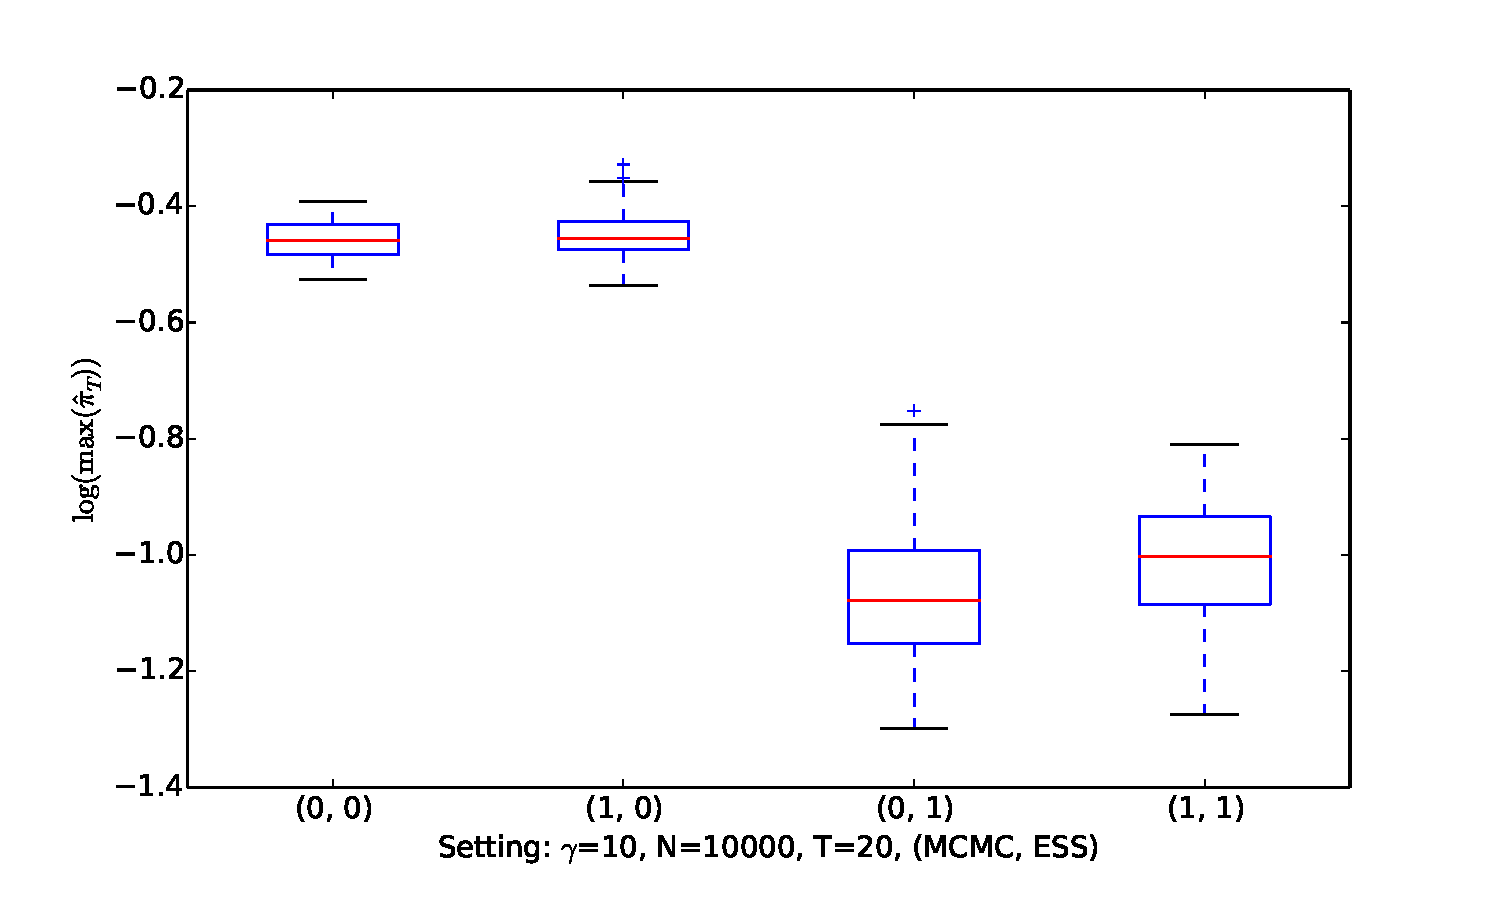
\includegraphics[width=\textwidth]{loglik_mcmc_ess/T20_gamma10_N10000.pdf}
      
    \end{minipage}%
    \begin{minipage}{0.5\textwidth}
        \centering
        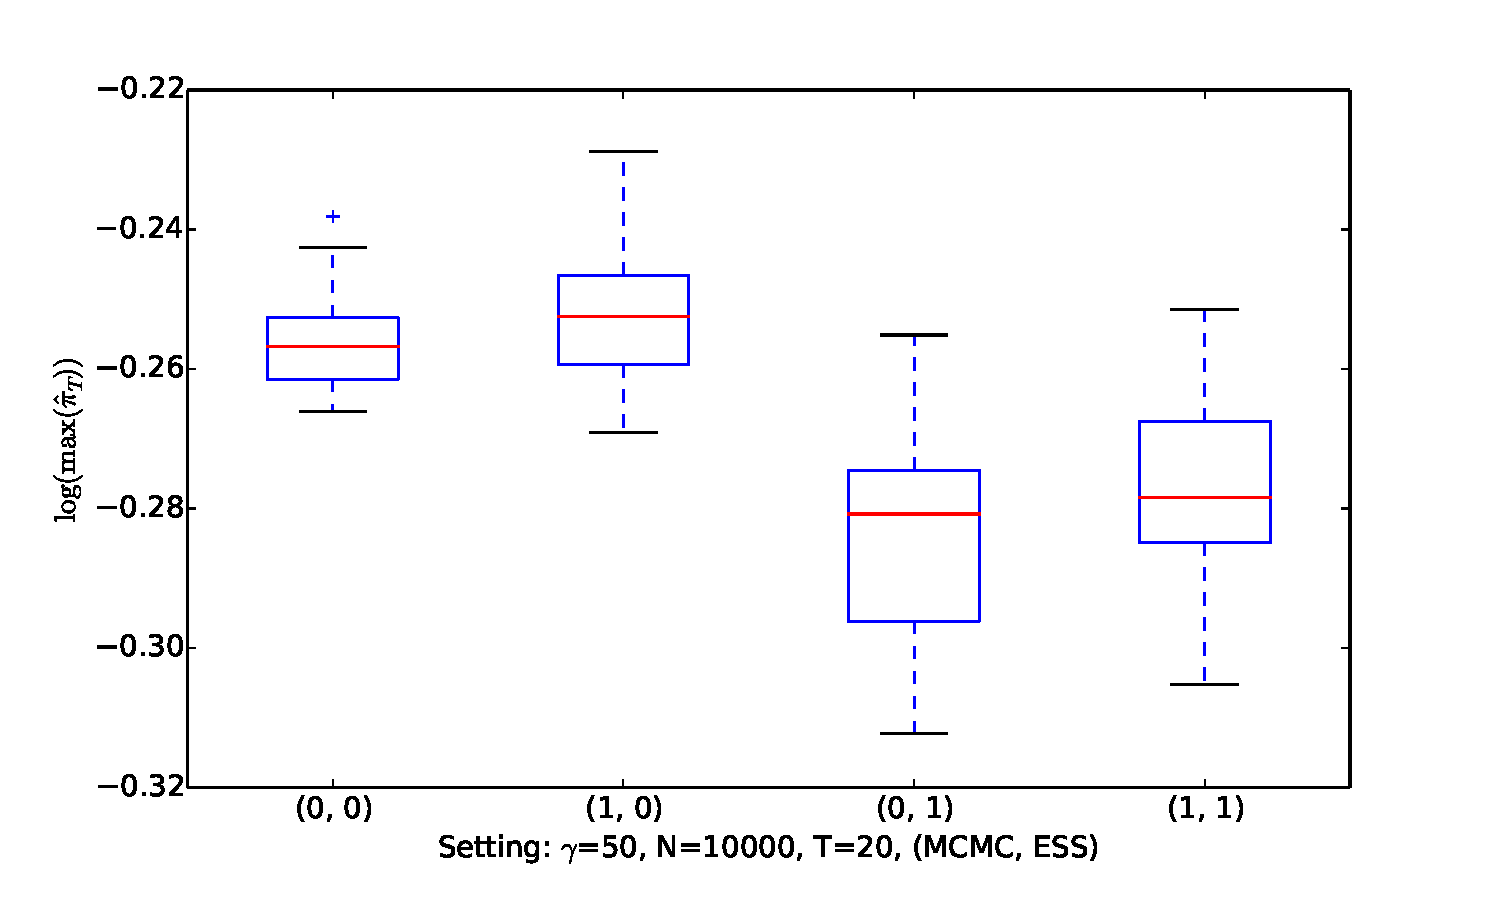
\includegraphics[width=\textwidth]{loglik_mcmc_ess/T20_gamma50_N10000.pdf}
      
    \end{minipage}
    \begin{minipage}{0.5\textwidth}
        \centering
        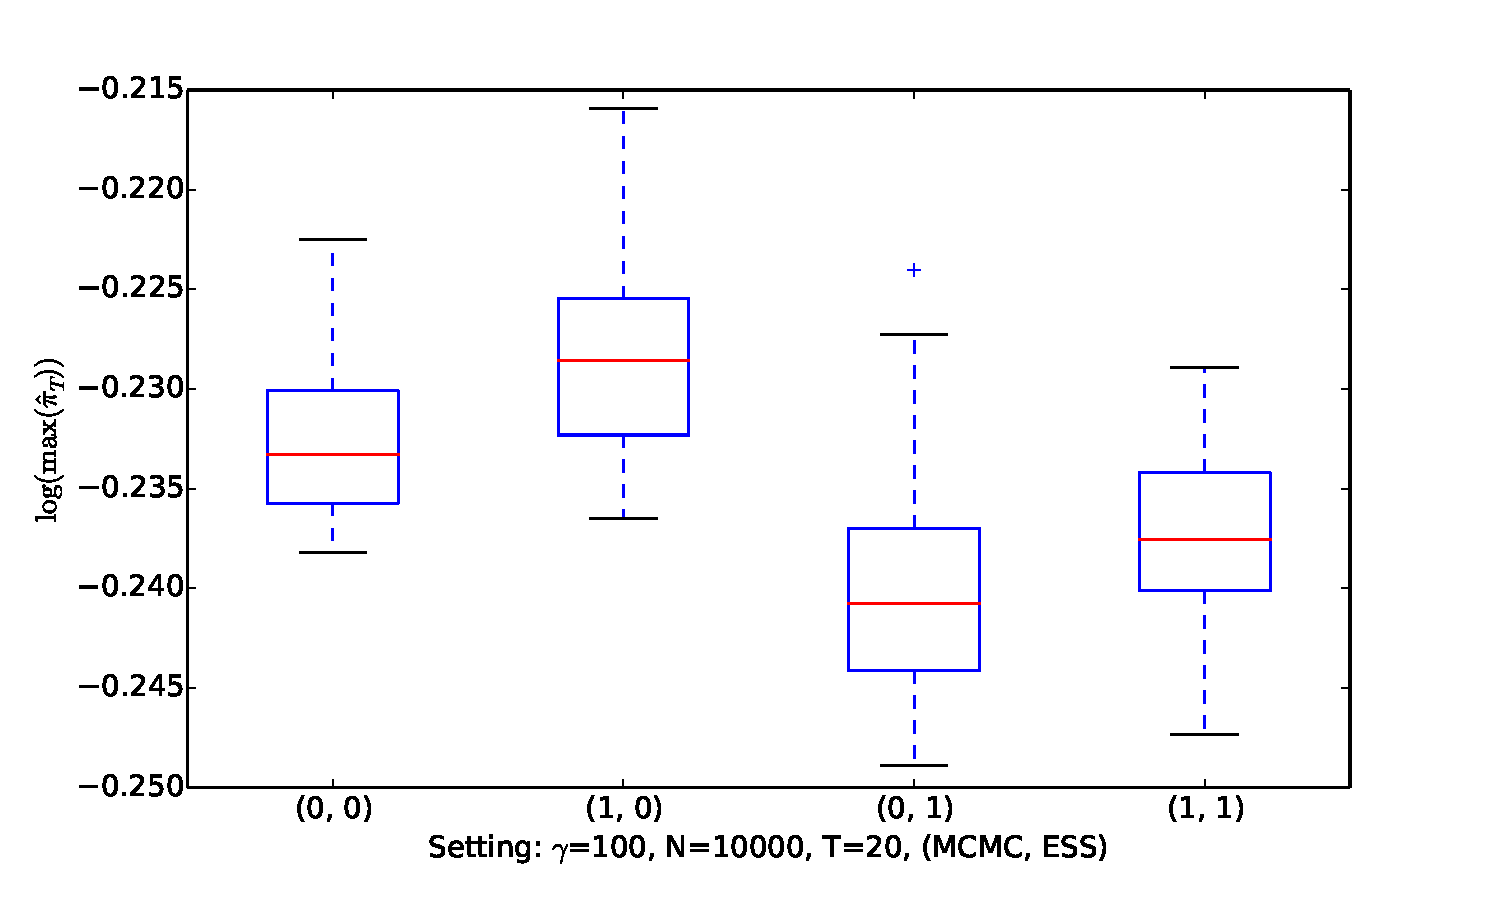
\includegraphics[width=\textwidth]{loglik_mcmc_ess/T20_gamma100_N10000.pdf}
      
    \end{minipage}%
    \begin{minipage}{0.5\textwidth}
        \centering
        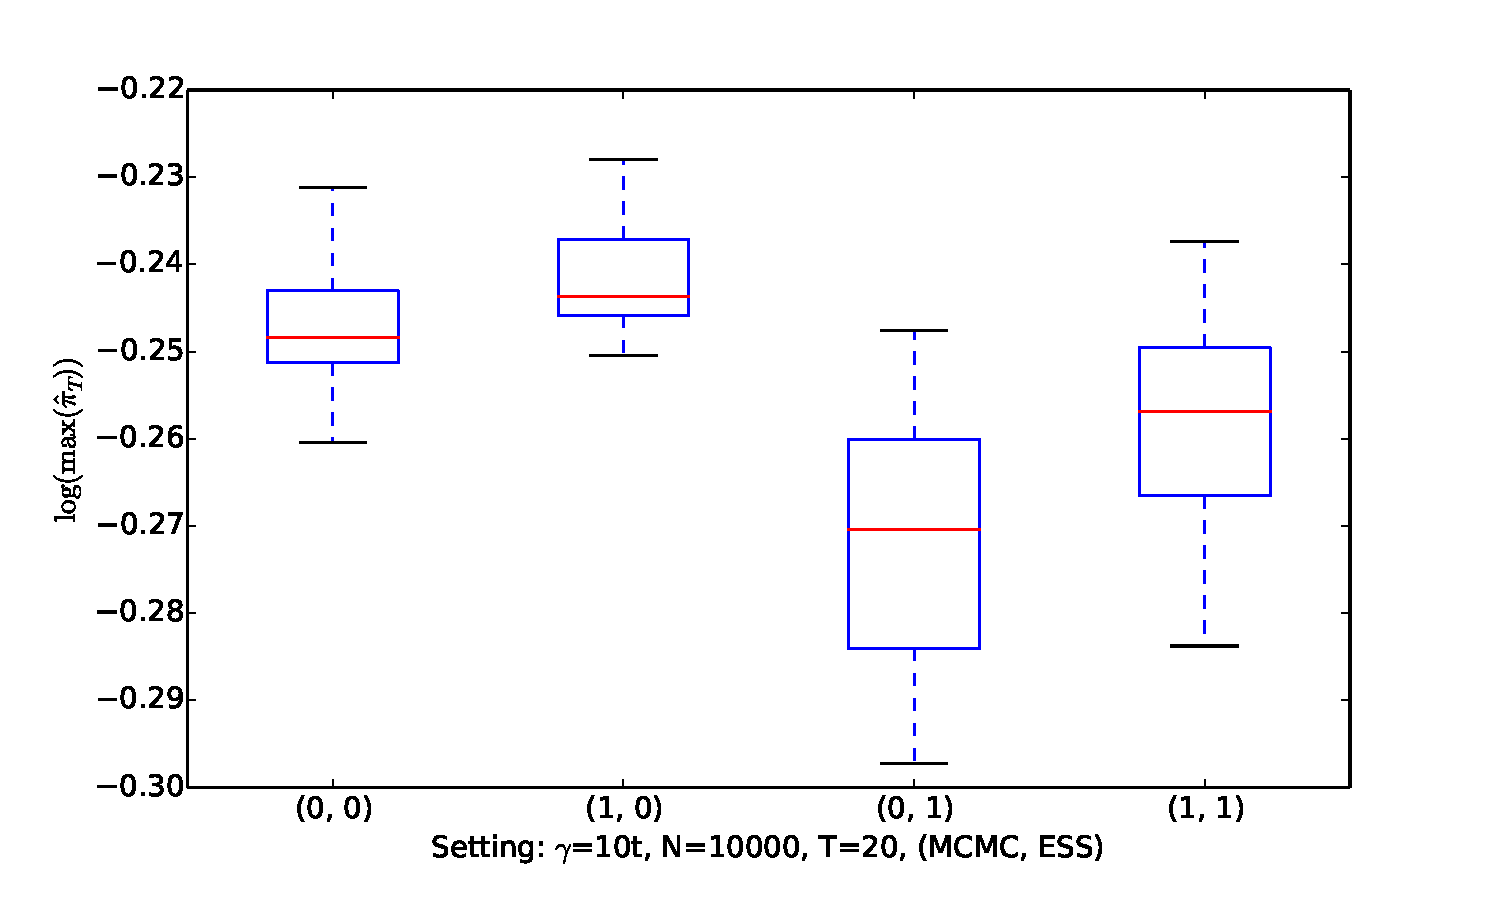
\includegraphics[width=\textwidth]{loglik_mcmc_ess/T20_gamma10t_N10000.pdf}
      
    \end{minipage}
    \begin{minipage}{0.5\textwidth}
        \centering
        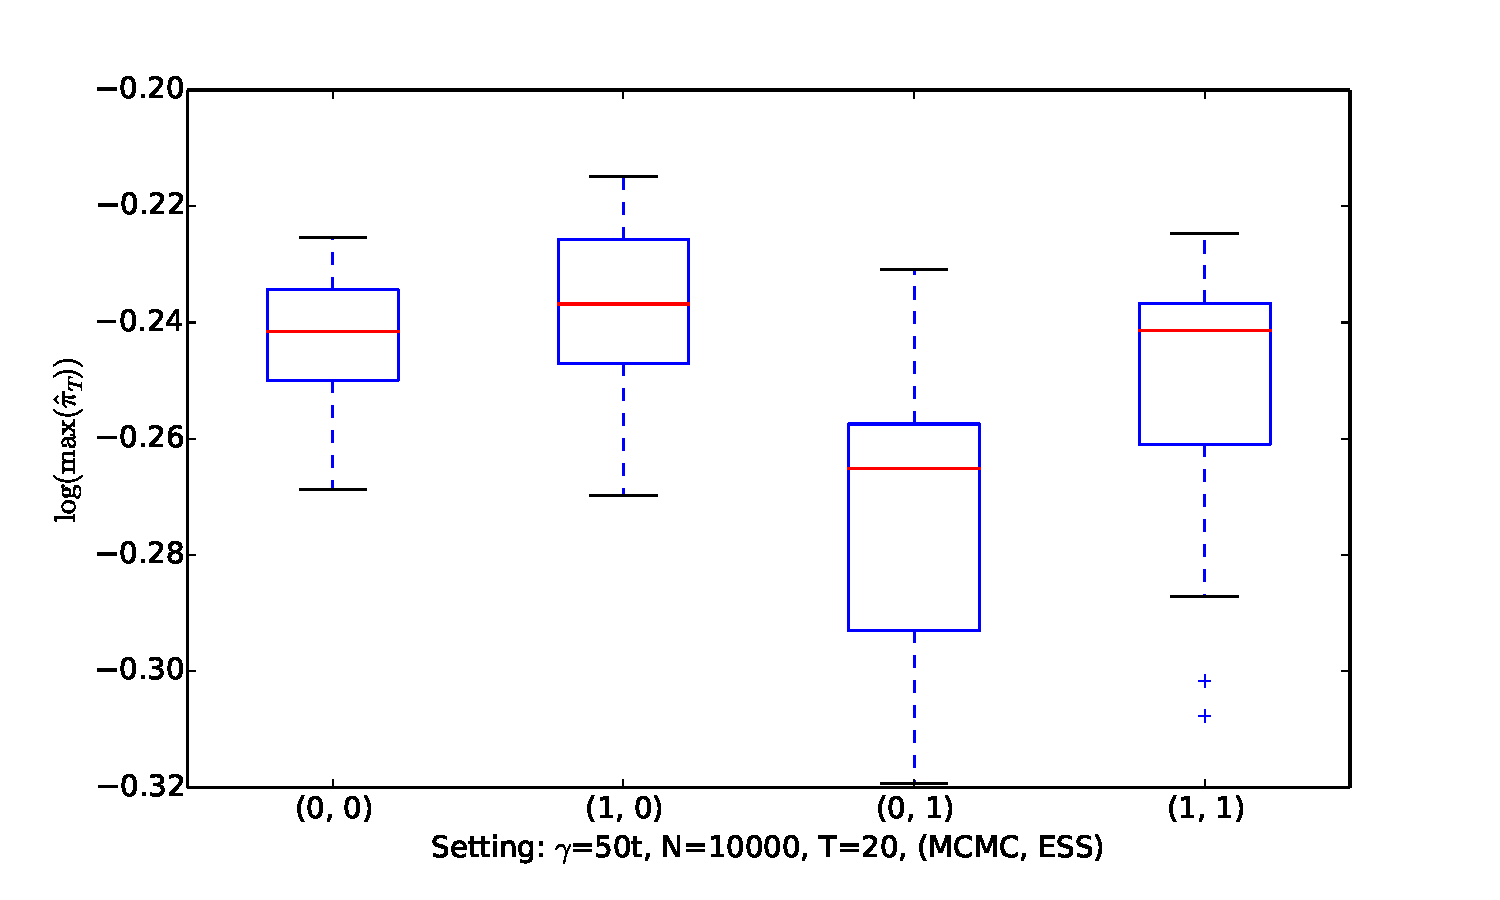
\includegraphics[width=\textwidth]{loglik_mcmc_ess/T20_gamma50t_N10000.pdf}
      
    \end{minipage}%
    \begin{minipage}{0.5\textwidth}
        \centering
        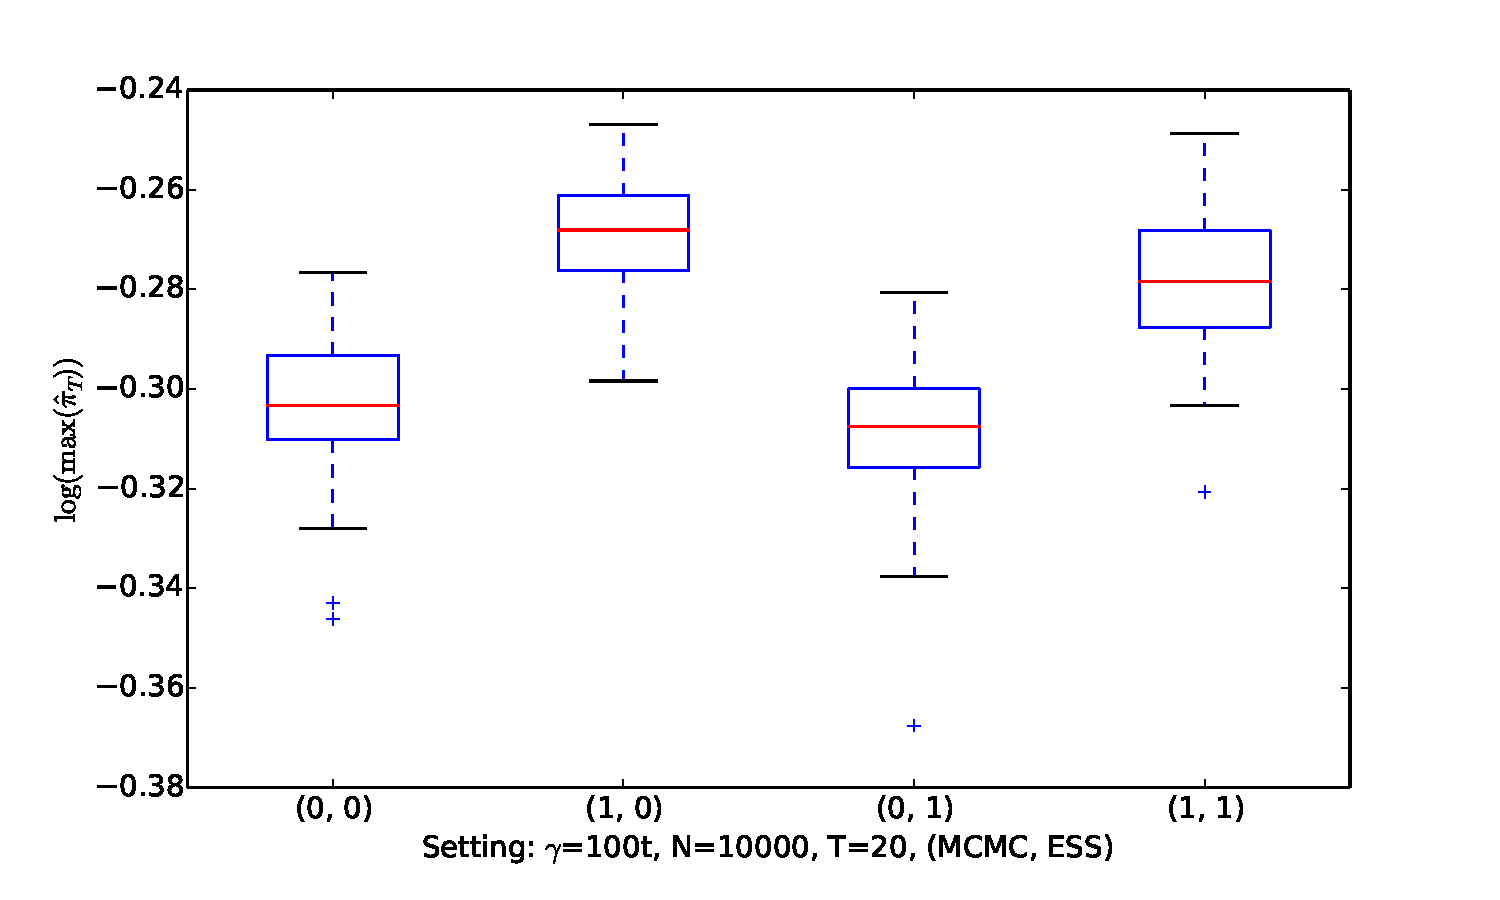
\includegraphics[width=\textwidth]{loglik_mcmc_ess/T20_gamma100t_N10000.pdf}
    \end{minipage}
    \caption{The performance in terms of $\log\pi_T(\hat{u}^*_{1:t})$ of 30 independent runs of the algorithms  with $T=20$ and $N=10000$ for various $\gamma$ settings. The four box-plots in each sub-figure represent the results of runs with the following settings (from left to right): a) MCMC disabled, ESS disabled, b) MCMC enabled, ESS disabled, c) MCMC disabled, ESS enabled, and d) MCMC enabled, ESS enabled.   }
    \label{fig:ess}
\end{figure}

\subsubsection{Resample-Move step with MCMC}
In Figure \ref{fig:ess}, we can also observe that the Resample-Move step does improve performance, albeit the improvement is marginal  in most of the cases. It is also found that the improvement is more significant when $\gamma$ is set to be high. Figure \ref{fig:rm1}, Figure \ref{fig:rm2} and Figure\ref{fig:rm3} show the box plots of $\log\pi_T(\hat{u}^*_{1:t})$ of $30$ independent runs for time period $T$ of 5, 10, 20 respectively. Each sub-figure shows the runs for a selected $\gamma$ setting with the box-plots grouped by whether the Resample-Move step is used (the leftmost 5 box-plots) or not (the rightmost 5 box-plots), sorted in terms of number of samples used $N$.

One possible explanation to this result is that high $\gamma$ settings sharpen the distribution shape. Such a setting encourages optimisation by pushing the sample towards  high density area but at the same time reduces the state space exploration. With excessively high $\gamma$ settings, the sample set may be led to a local optimal with relatively high density area, but may not be the mode of the distribution. The perturbation that Resample-Move step introduced at each iteration may help particles to escape from local optimal.

\begin{figure}[!thbp]
    \centering
    \begin{minipage}{.5\textwidth}
        \centering
        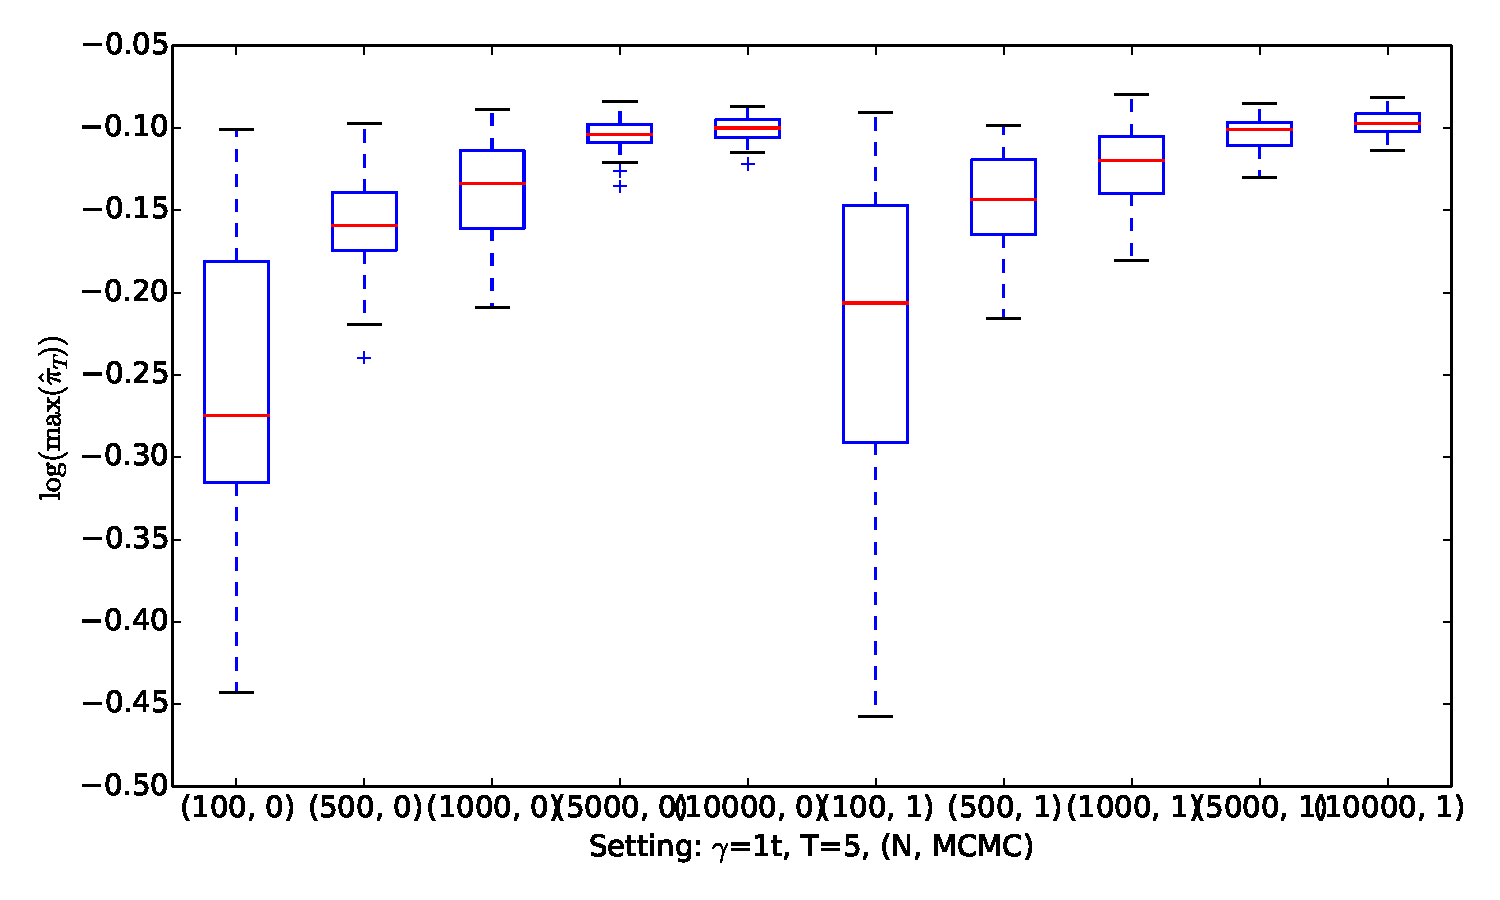
\includegraphics[width=\textwidth]{loglik_t_gs_n/T5_gamma1t.pdf}
    \end{minipage}%
    \begin{minipage}{0.5\textwidth}
        \centering
        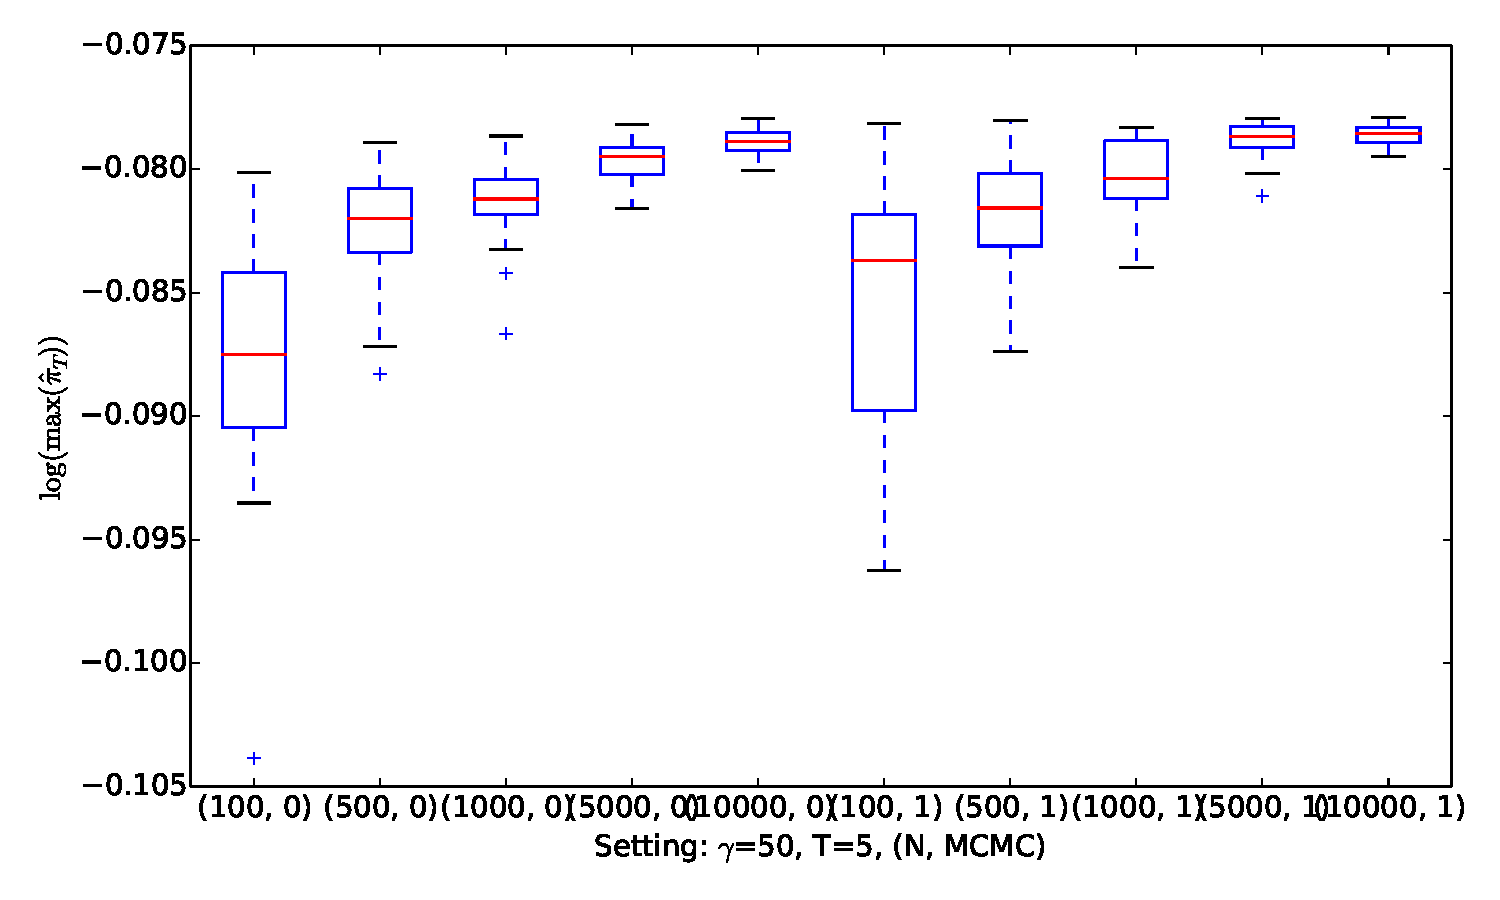
\includegraphics[width=\textwidth]{loglik_t_gs_n/T5_gamma50.pdf}
    \end{minipage}
    \begin{minipage}{0.5\textwidth}
        \centering
        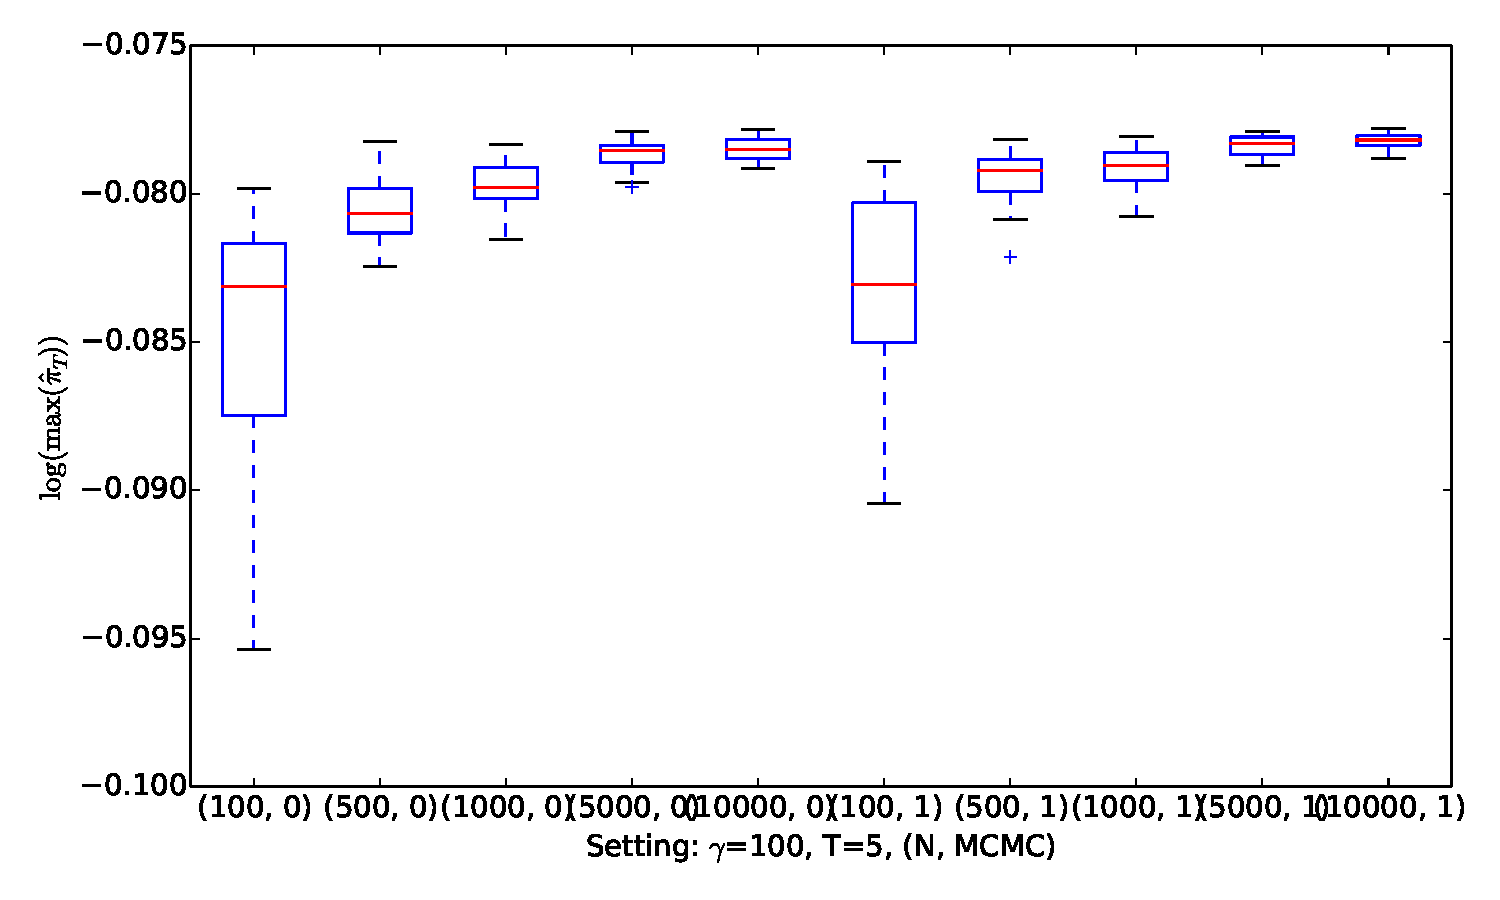
\includegraphics[width=\textwidth]{loglik_t_gs_n/T5_gamma100.pdf}
    \end{minipage}%
    \begin{minipage}{0.5\textwidth}
        \centering
        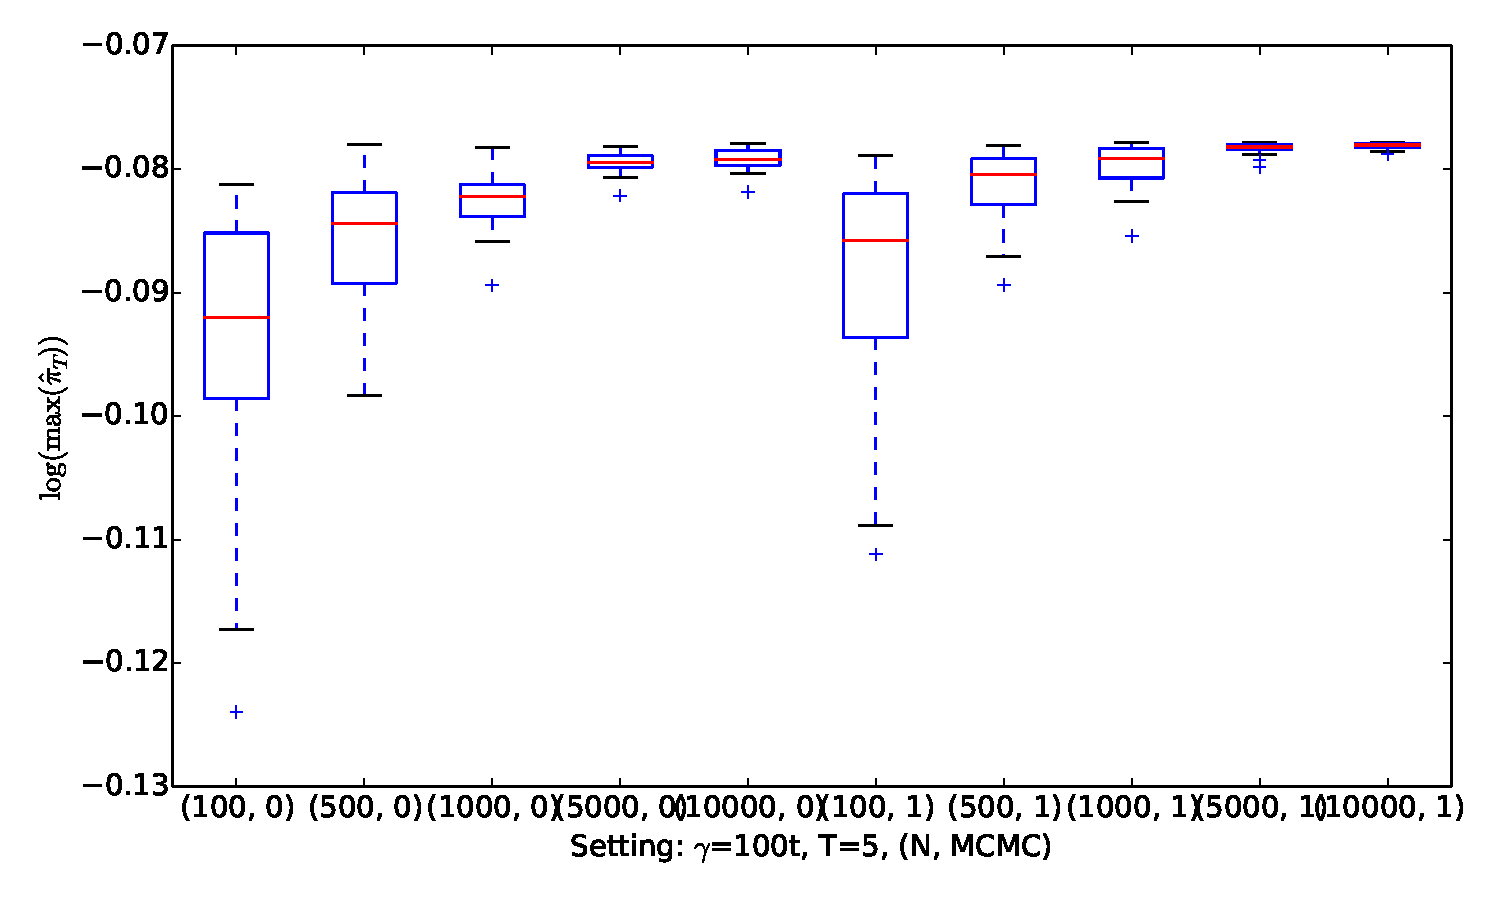
\includegraphics[width=\textwidth]{loglik_t_gs_n/T5_gamma100t.pdf}
    \end{minipage}
    \caption{The $\log\pi_T(\hat{u}^*_{1:t})$ box-plots of 30 independent runs with various settings for $T=5$. Each sub-figure shows the runs for a selected $\gamma$ setting with the box-plots grouped by whether the Resample-Move step is used (the leftmost 5 box-plots) or not (the rightmost 5 box-plots), sorted in terms of number of samples used $N$.}
    \label{fig:rm1}
\end{figure}

\begin{figure}[!thbp]
    \centering
    \begin{minipage}{0.5\textwidth}
        \centering
        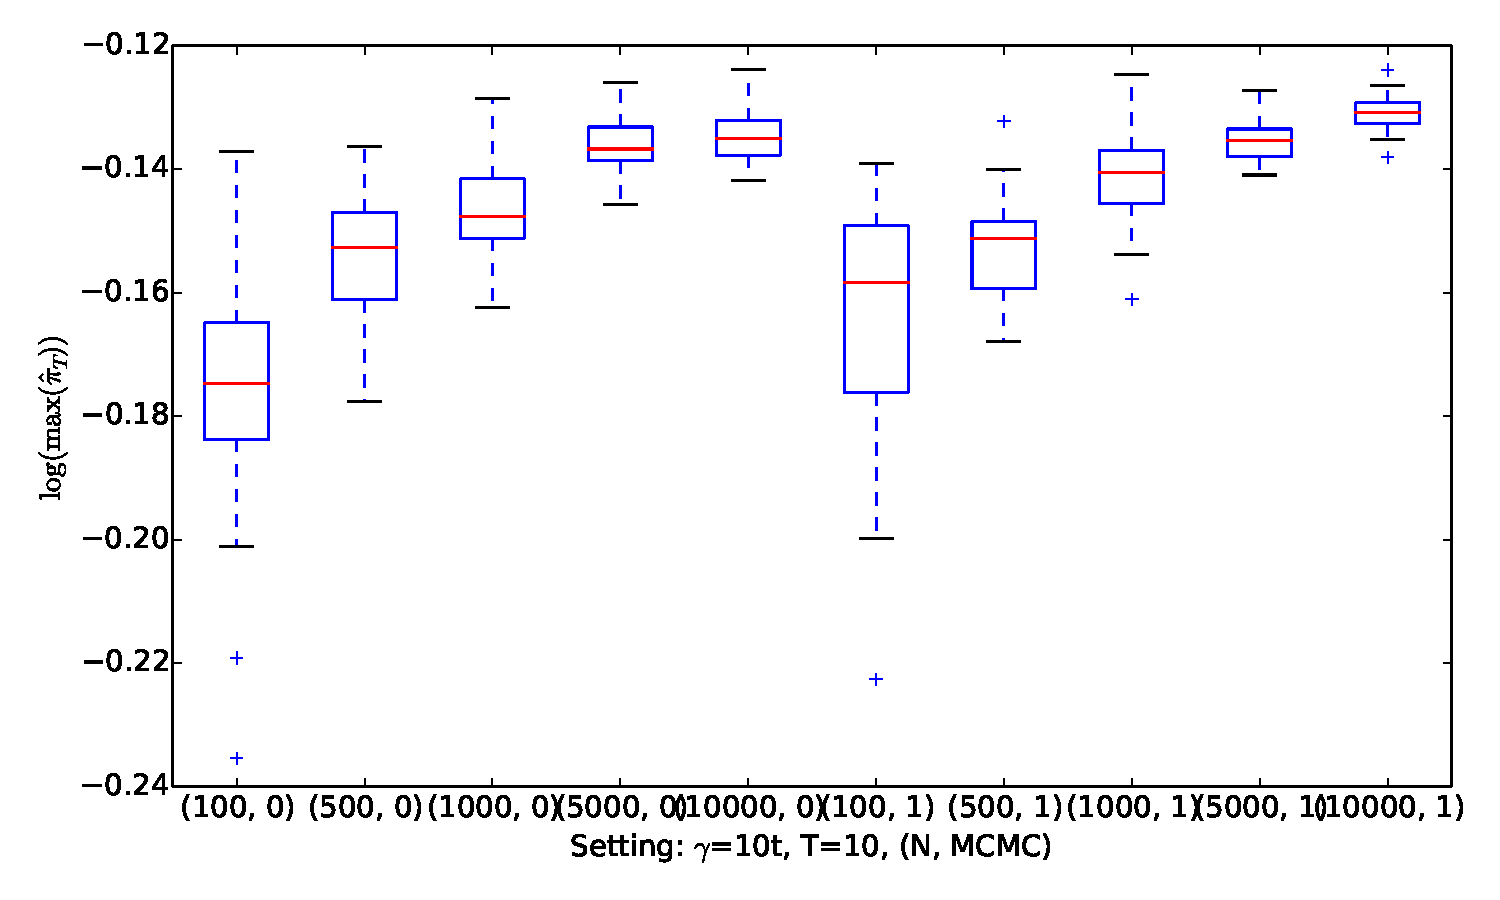
\includegraphics[width=\textwidth]{loglik_t_gs_n/T10_gamma10t.pdf}
    \end{minipage}%
    \begin{minipage}{0.5\textwidth}
        \centering
        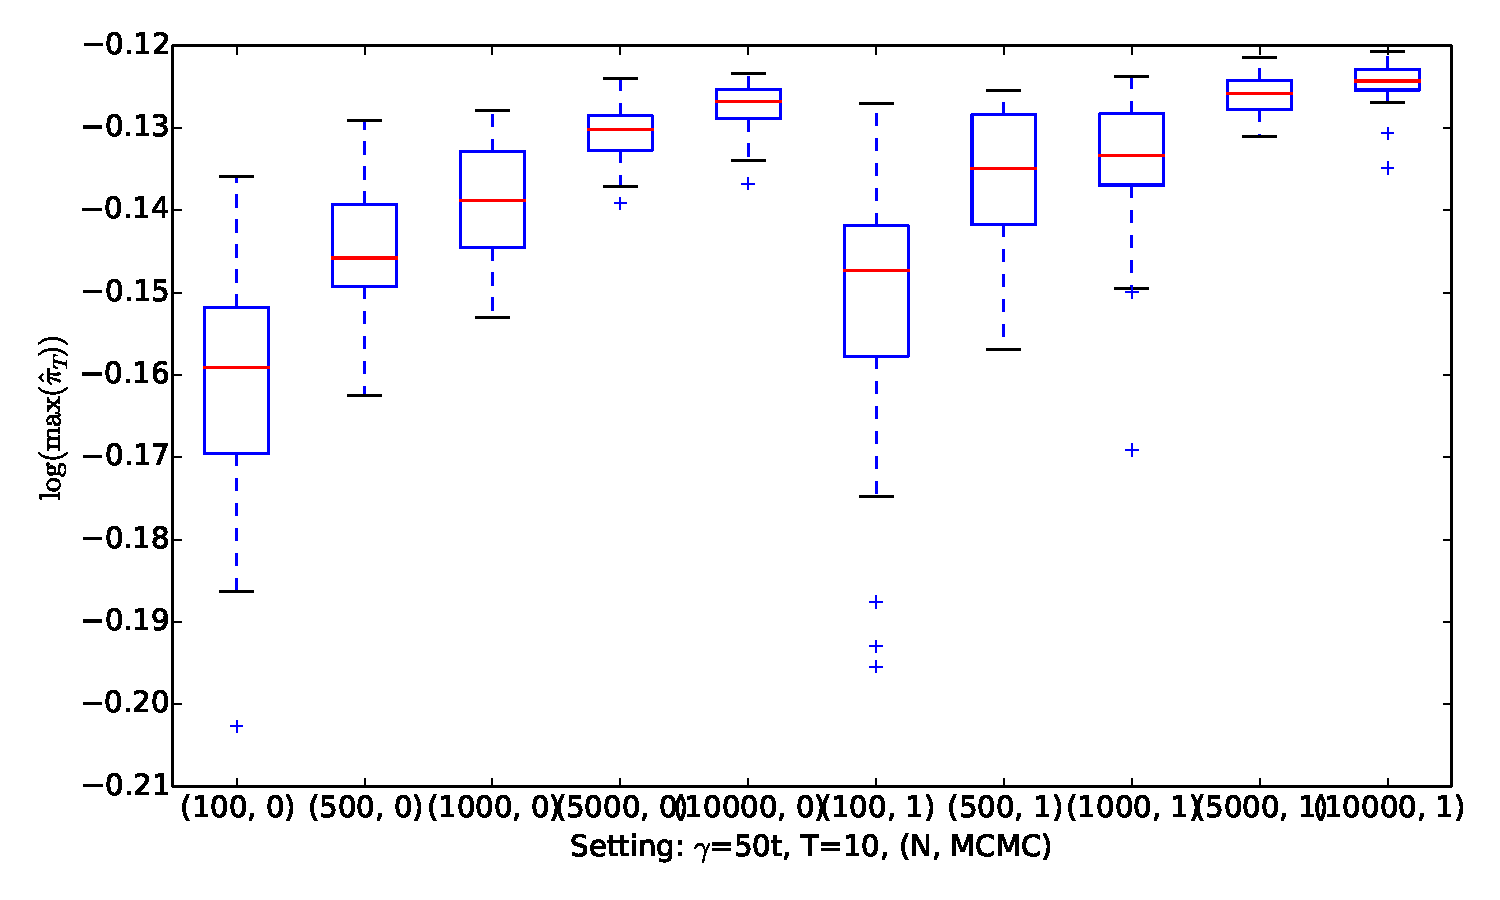
\includegraphics[width=\textwidth]{loglik_t_gs_n/T10_gamma50t.pdf}
    \end{minipage}
    \begin{minipage}{0.5\textwidth}
        \centering
        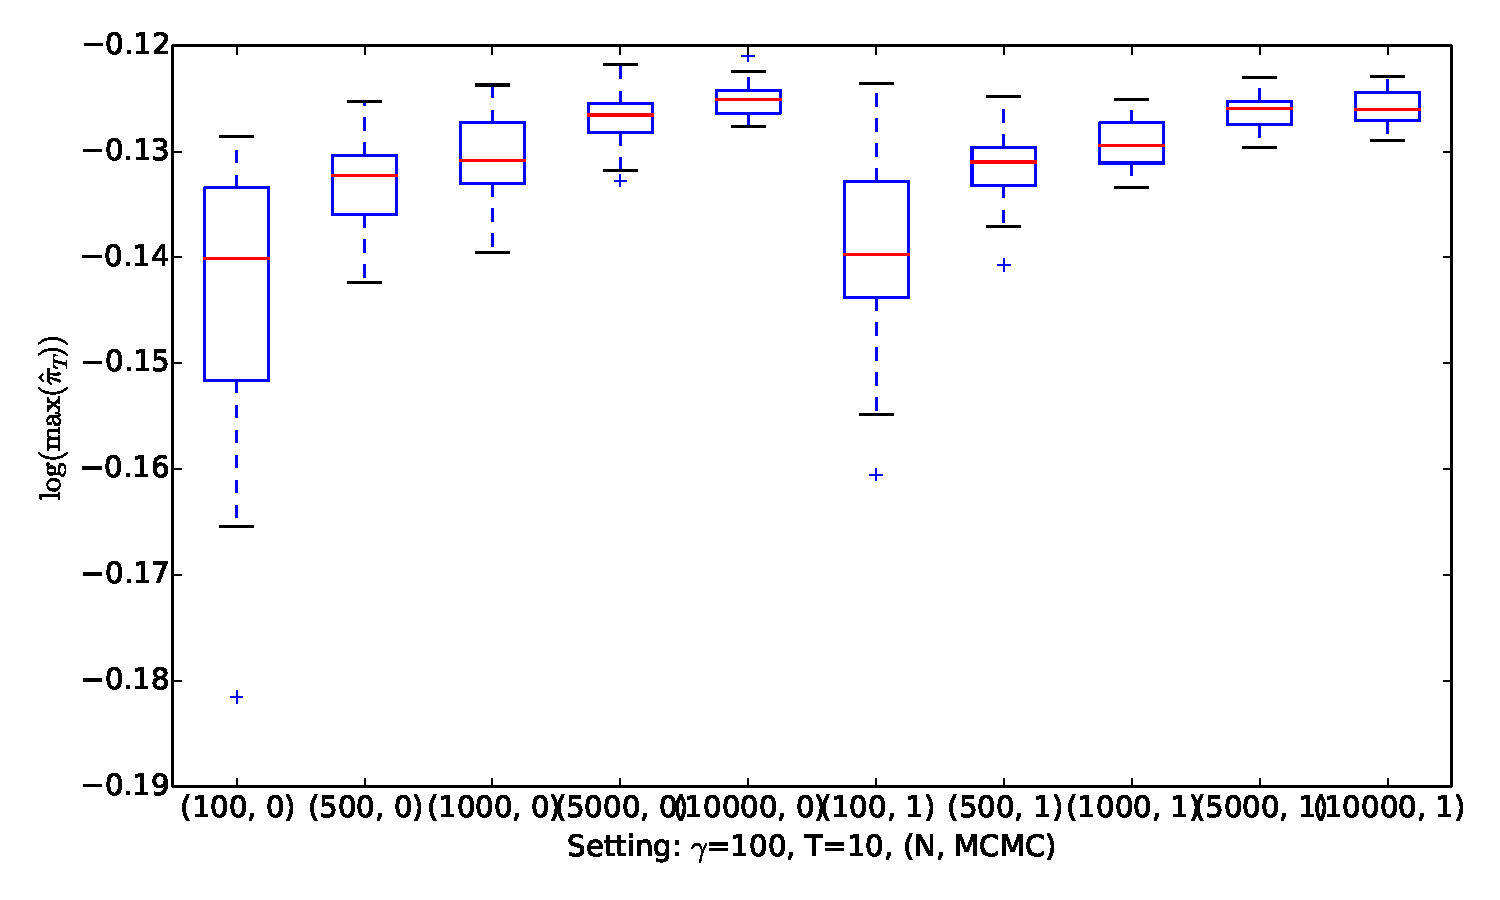
\includegraphics[width=\textwidth]{loglik_t_gs_n/T10_gamma100.pdf}
    \end{minipage}%
    \begin{minipage}{0.5\textwidth}
        \centering
        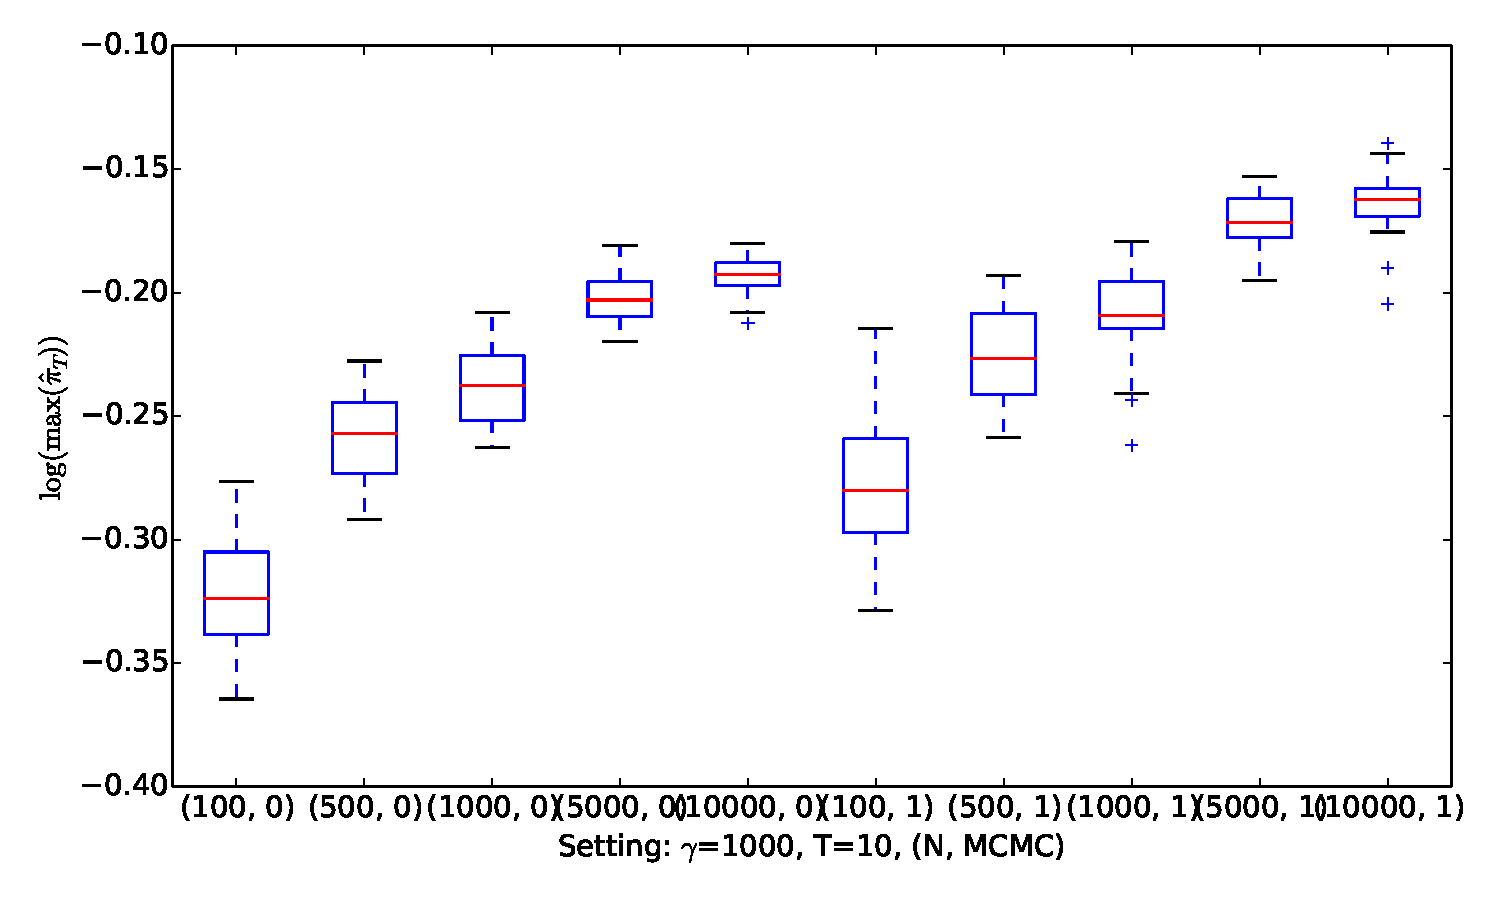
\includegraphics[width=\textwidth]{loglik_t_gs_n/T10_gamma1000.pdf}
    \end{minipage}
    \caption{The $\log\pi_T(\hat{u}^*_{1:t})$ box-plots of 30 independent runs with various settings for $T=10$. Each sub-figure shows the runs for a selected $\gamma$ setting with the box-plots grouped by whether the Resample-Move step is used (the leftmost 5 box-plots) or not (the rightmost 5 box-plots), sorted in terms of number of samples used $N$.}
    \label{fig:rm2}
\end{figure}

\begin{figure}[!thbp]
    \centering
    \begin{minipage}{0.5\textwidth}
        \centering
        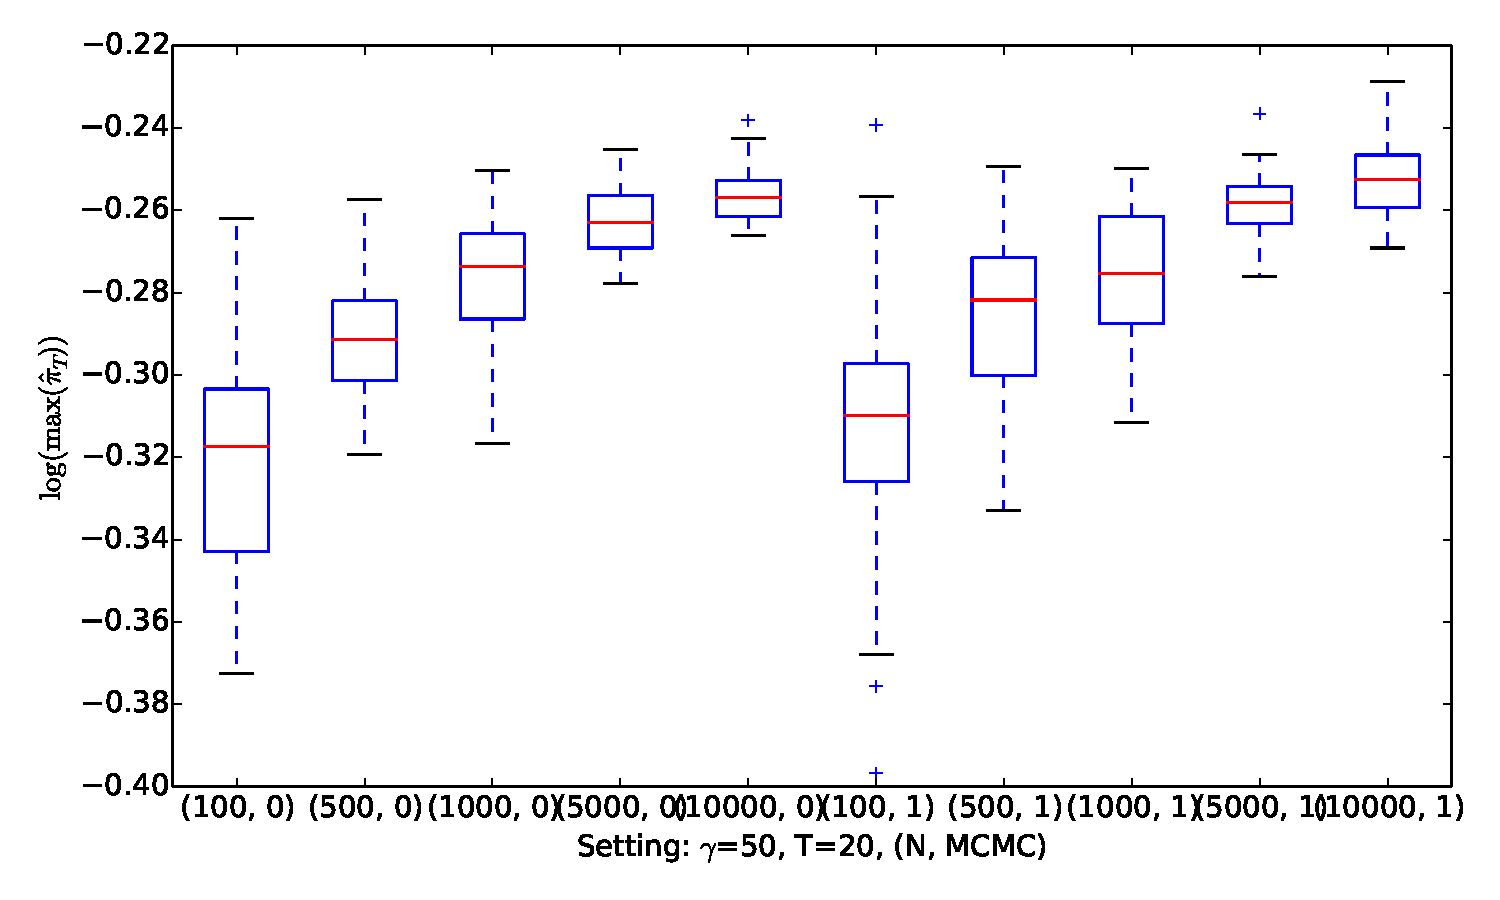
\includegraphics[width=\textwidth]{loglik_t_gs_n/T20_gamma50.pdf}
    \end{minipage}%
    \begin{minipage}{0.5\textwidth}
        \centering
        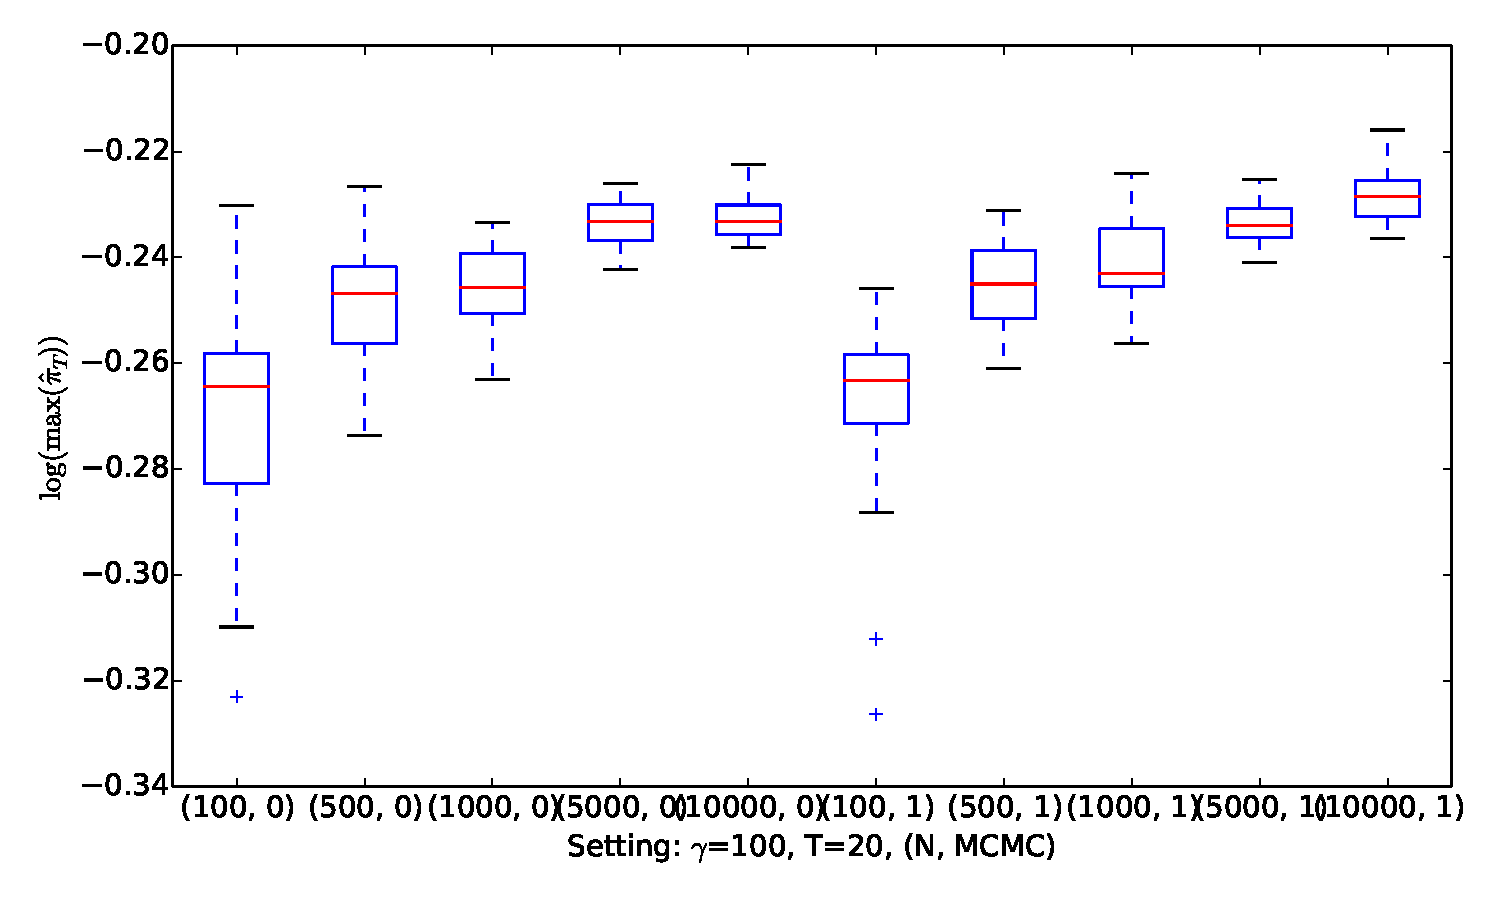
\includegraphics[width=\textwidth]{loglik_t_gs_n/T20_gamma100.pdf}
    \end{minipage}
    \begin{minipage}{0.5\textwidth}
        \centering
        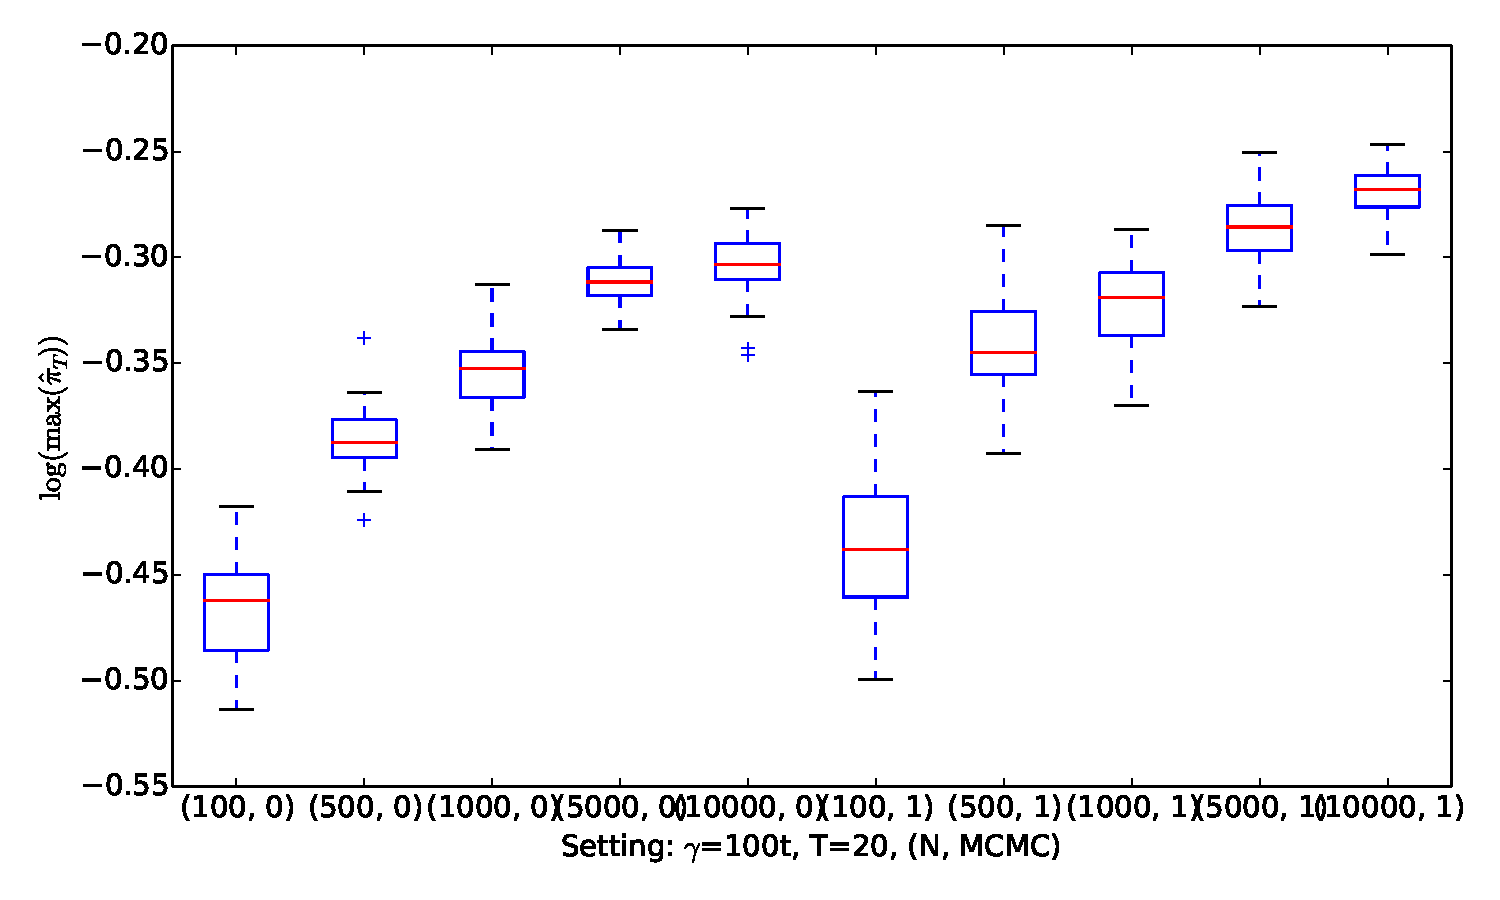
\includegraphics[width=\textwidth]{loglik_t_gs_n/T20_gamma100t.pdf}
    \end{minipage}%
    \begin{minipage}{0.5\textwidth}
        \centering
        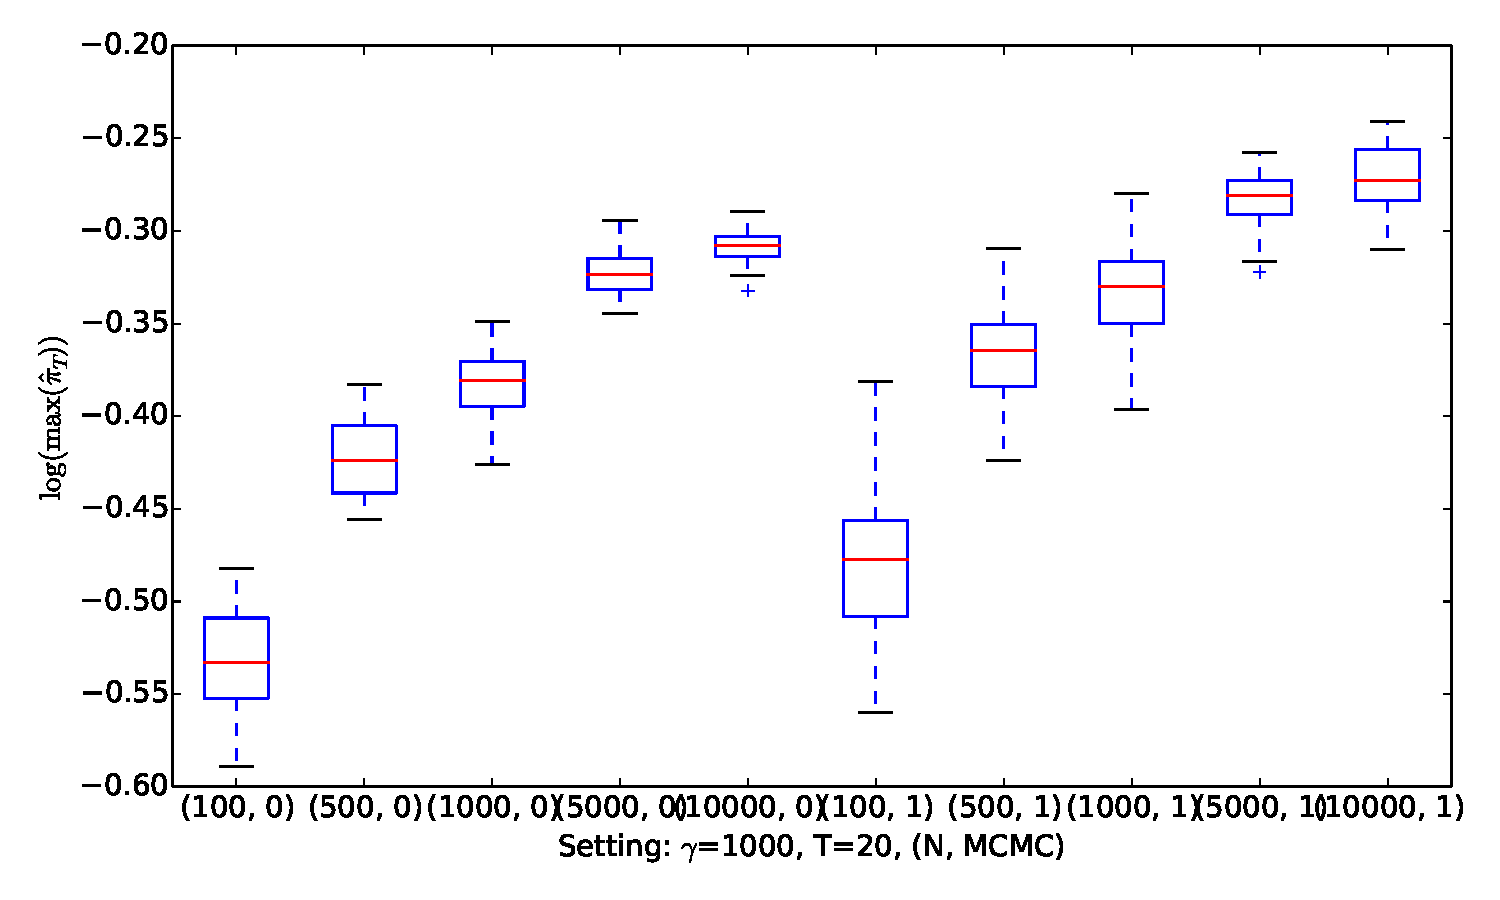
\includegraphics[width=\textwidth]{loglik_t_gs_n/T20_gamma1000.pdf}
    \end{minipage}
    \caption{The $\log\pi_T(\hat{u}^*_{1:t})$ box-plots of 30 independent runs with various settings for $T=20$. Each sub-figure shows the runs for a selected $\gamma$ setting with the box-plots grouped by whether the Resample-Move step is used (the leftmost 5 box-plots) or not (the rightmost 5 box-plots), sorted in terms of number of samples used $N$.}
    \label{fig:rm3}
\end{figure}

\subsubsection{Various sample size settings}
In terms of the sample size setting used, the performance increased monotonically with the number of samples used for all time periods. This can seen clearly from the box-plots shown in Figure \ref{fig:rm1}, Figure \ref{fig:rm2} and Figure \ref{fig:rm3}. This is in-line with the theory that more samples is always better. For the shorter time-period considered, says $T=5$, the performance improvement sometimes is ``saturated'' even with lower number of samples, says $T=1000$ or $T=5000$. This suggests the optimal control parameters may have been attained.

 \subsubsection{Various $\gamma$ settings}
A more interesting result is to compare the performance with different $\gamma$ settings. Let first consider the fixed $\gamma$ settings. Excessive high $\gamma$ settings may lead to the issue discussed earlier and stuck at local optimal. On the other hand, low $\gamma$ settings also does not perform too well either (consider the process of searching for the mode by randomly sampling a very flat distribution). The optimal $\gamma$ setting seems to lie sometimes in between. In this case, the $\gamma=100$ setting results in the best performance.

In \cite{NK11}, it was suggested that using an increasing $\gamma$ setting may be a good pragmatic compromise between accuracy and good mixing. We investigate further on this by setting $\gamma$ to be increasing function of the form $\alpha t$, where $\alpha$ is constant and $t$ is the time step. The results show that the performance seems to be reasonably good when the $\alpha$ value is set low, but  worse when the $\alpha$ value is set too high. This suggests a capping on the maximum value on $\alpha$ or a more moderate increase in $t$ may be more suitable. We therefore carry out two extra $\gamma$ settings: $50\log(t+1)$ and $100\log(t+1)$ to investigate this. The results of these runs are shown in Figure \ref{fig:log}. The results from these runs look good but they are not statistically different from a simple fixed $\gamma=100$ setting.

\begin{figure}[!thbp]
    \centering
    \begin{minipage}{.5\textwidth}
        \centering
        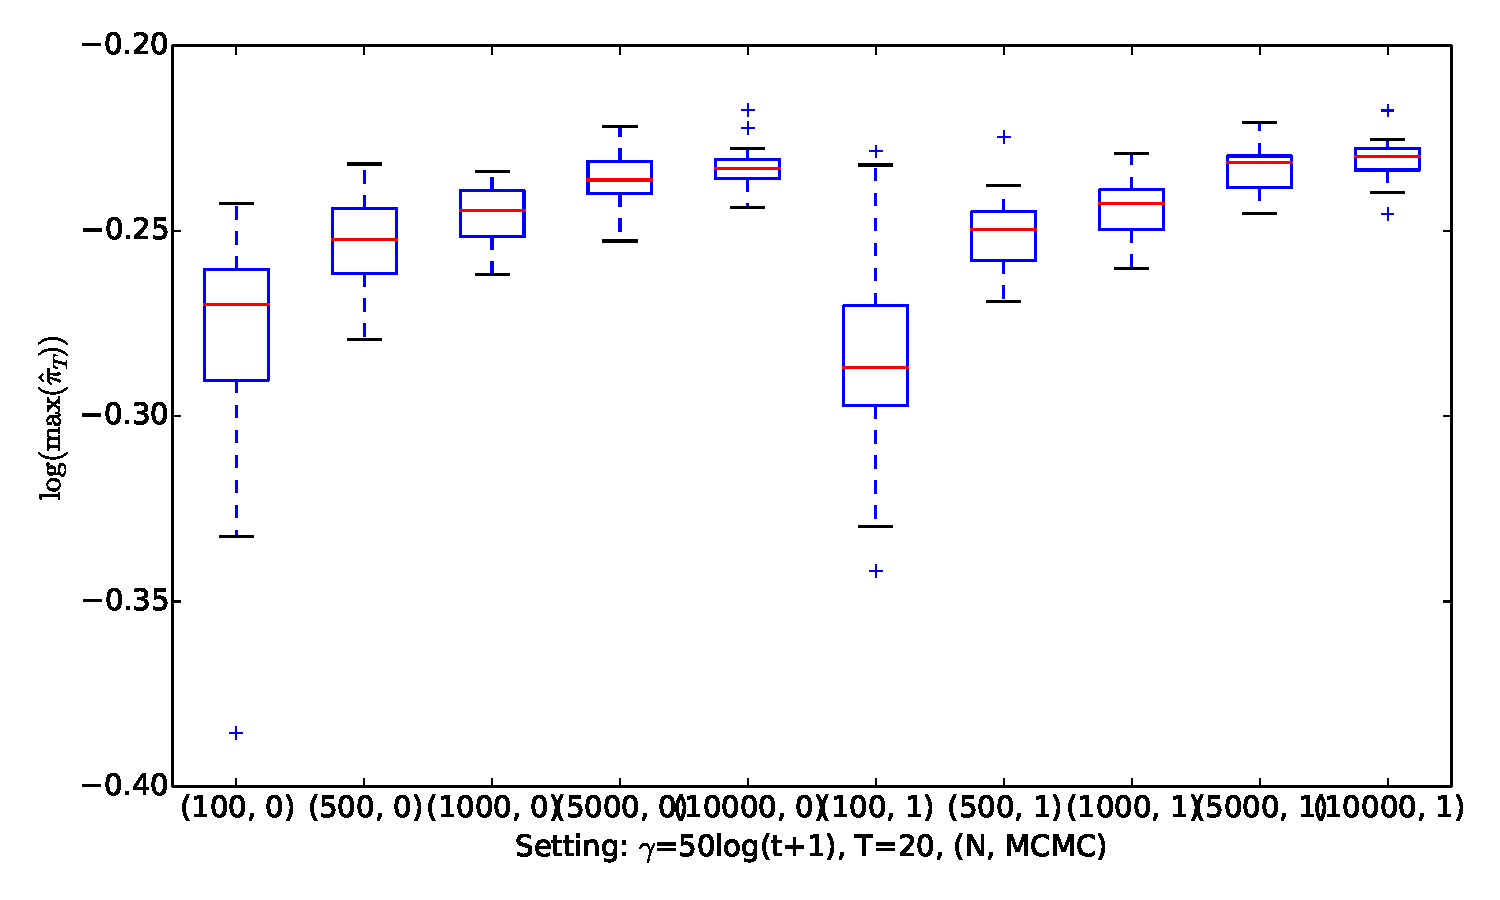
\includegraphics[width=\textwidth]{loglik_t_gs_n/T20_gamma50log(t+1).pdf}
        %\includegraphics[width=0.3\linewidth, height=0.15\textheight]{prob1_6_2}
        %\caption{$dt=0.1$}
        %\label{fig:prob1_6_2}
    \end{minipage}%
    \begin{minipage}{0.5\textwidth}
        \centering
        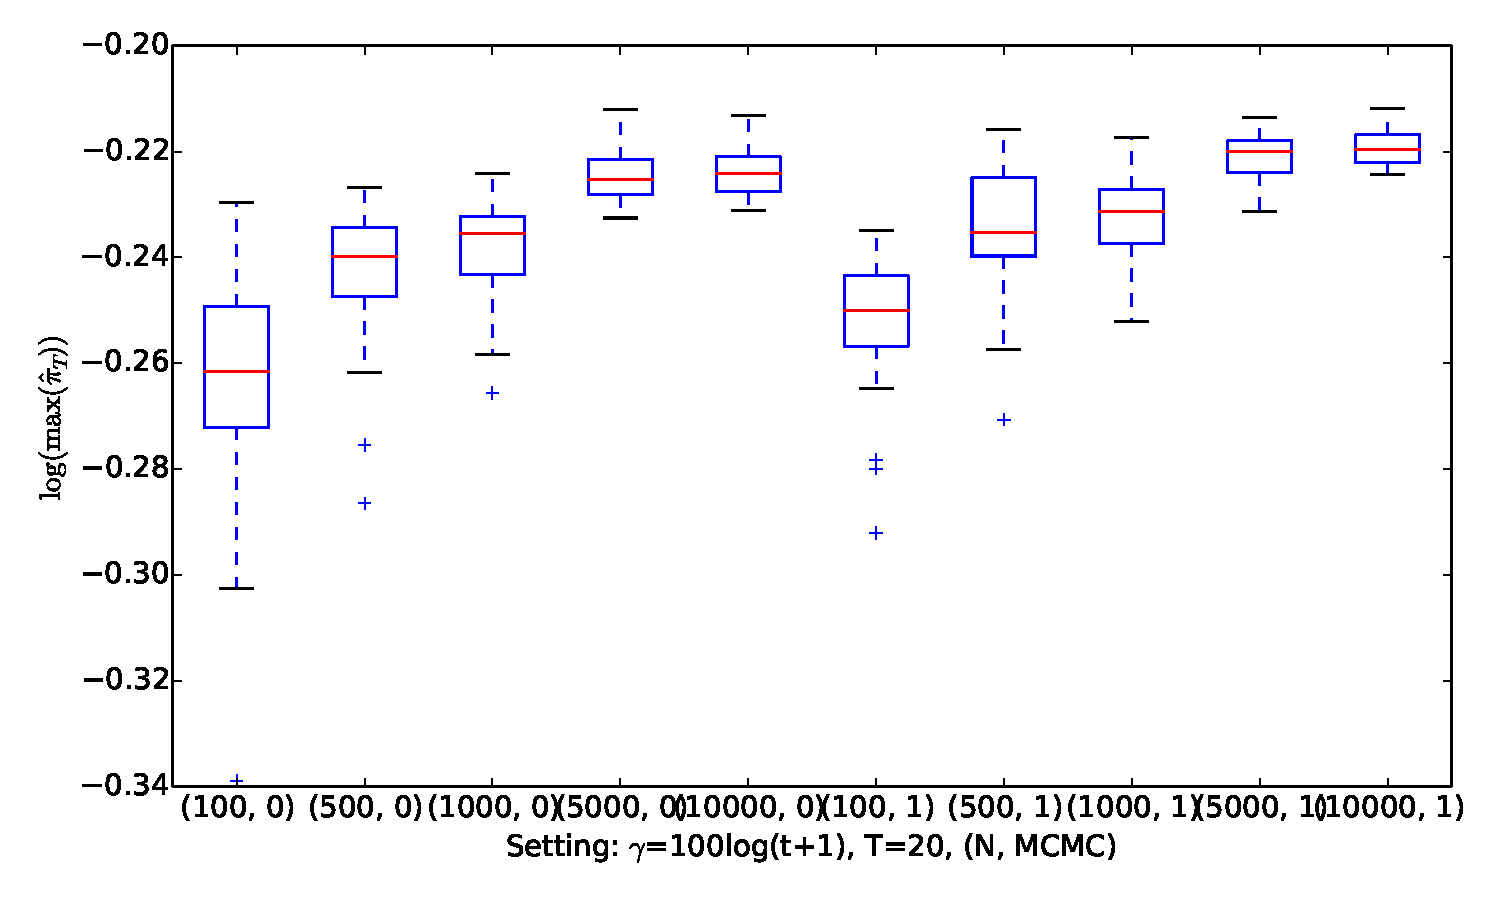
\includegraphics[width=\textwidth]{loglik_t_gs_n/T20_gamma100log(t+1).pdf}
    \end{minipage}
    \caption{The $\log\pi_T(\hat{u}^*_{1:t})$ box-plots of 30 independent runs with $\gamma$ settings: $50\log(t+1)$ and $100\log(t+1)$ and $T = 20$. Each sub-figure shows the runs for a selected $\gamma$ setting with the box-plots grouped by whether the Resample-Move step is used (the leftmost 5 box-plots) or not (the rightmost 5 box-plots), sorted in terms of number of samples used $N$.}
    \label{fig:log}
\end{figure}

Lastly, we conclude this section by showing the mean of the recursive likelihood $m_{t \mid t-1}(u^*_{1:T})$ obtained in various runs in Figure \ref{fig:estimatedy} and their corresponding tracking errors in Figure \ref{fig:error}. The results looks very promising. Except in the runs with the $\gamma=1$ setting in which there is a lot of noise in tracking, all other runs are able to closely track the reference signal. 

\begin{figure}[!thbp]
    \centering
    \begin{minipage}{.5\textwidth}
        \centering
        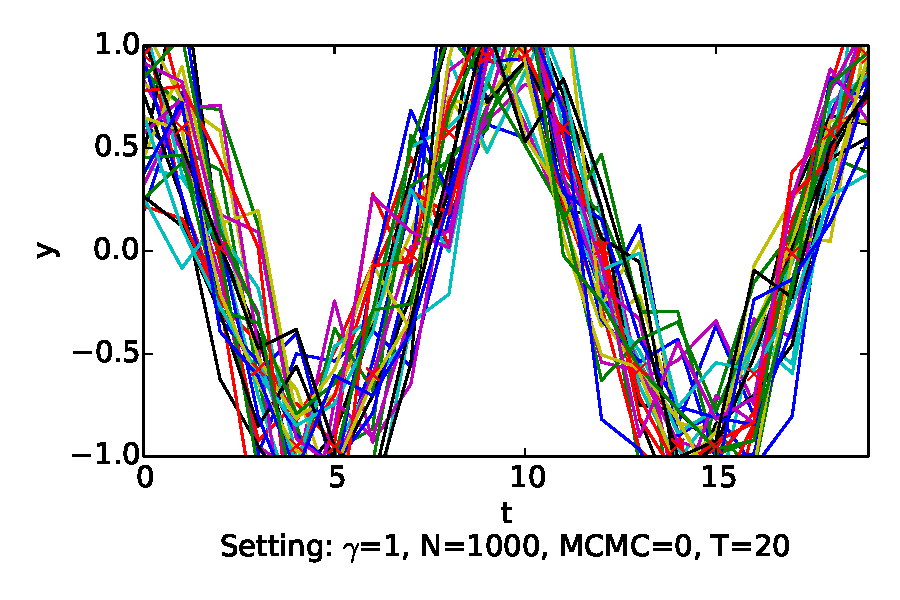
\includegraphics[width=\textwidth]{output_y/output_20_1.pdf}
    \end{minipage}%
    \begin{minipage}{0.5\textwidth}
        \centering
        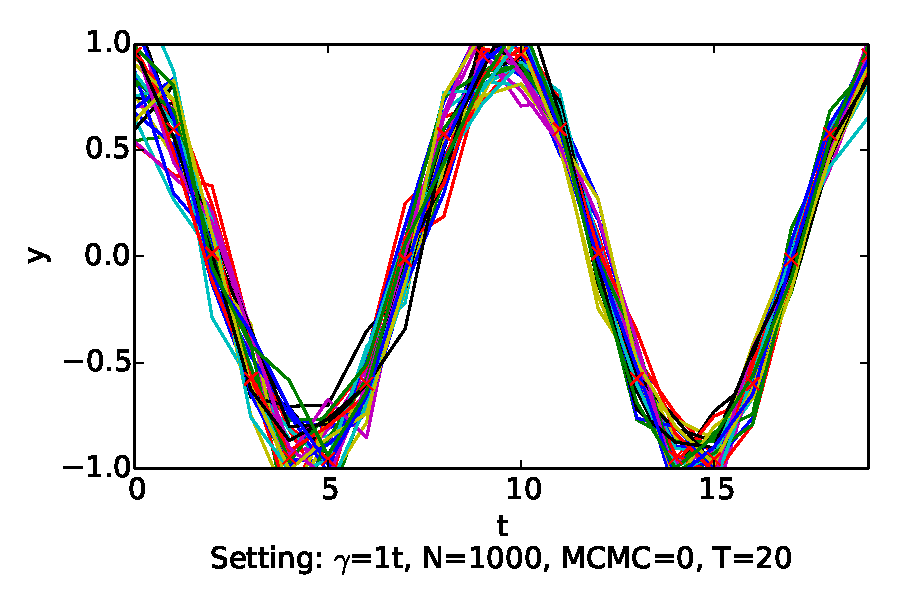
\includegraphics[width=\textwidth]{output_y/output_20_1t.pdf}
    \end{minipage}
    \begin{minipage}{0.5\textwidth}
        \centering
        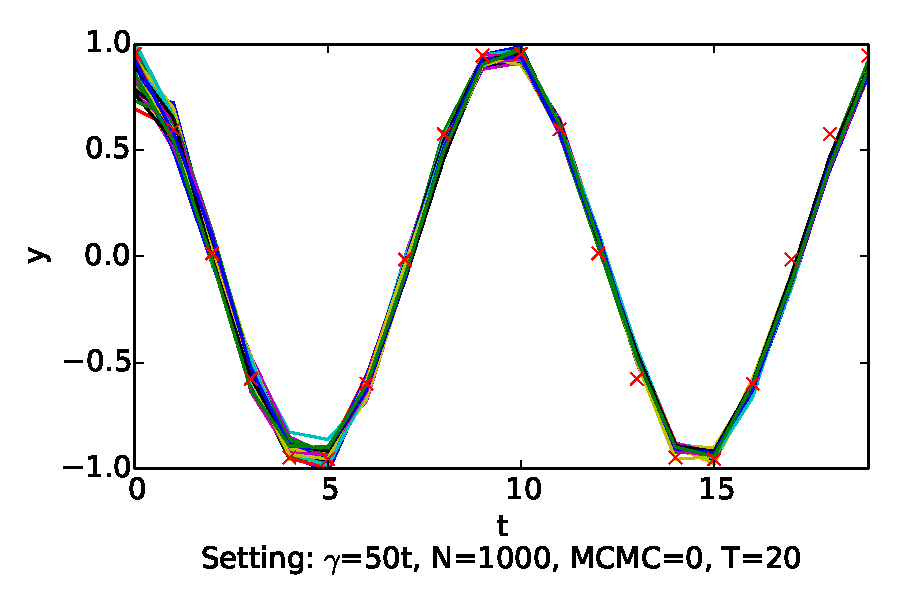
\includegraphics[width=\textwidth]{output_y/output_20_50t.pdf}
    \end{minipage}%
    \begin{minipage}{0.5\textwidth}
        \centering
        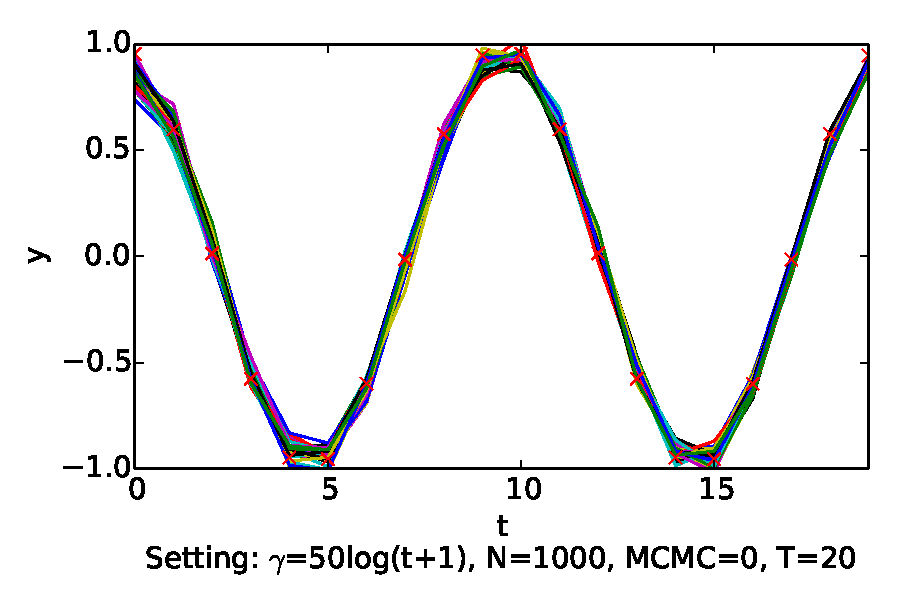
\includegraphics[width=\textwidth]{output_y/output_20_50log(t+1).pdf}
    \end{minipage}
    \begin{minipage}{0.5\textwidth}
        \centering
        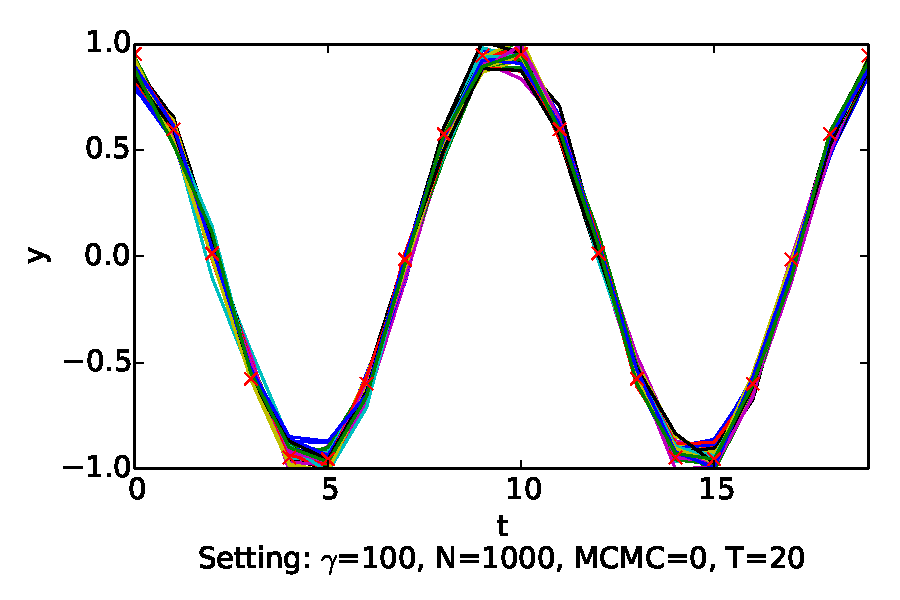
\includegraphics[width=\textwidth]{output_y/output_20_100.pdf}
    \end{minipage}%
    \begin{minipage}{0.5\textwidth}
        \centering
        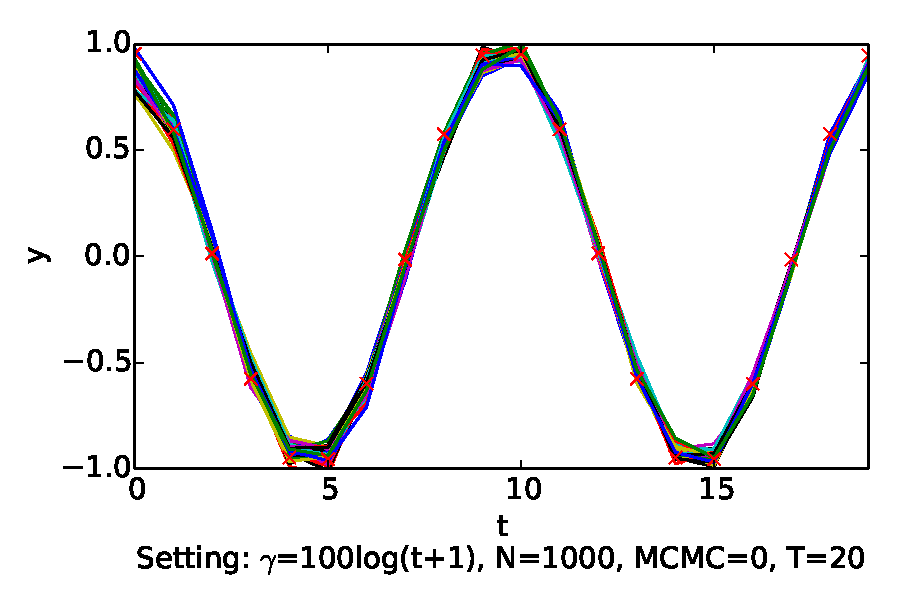
\includegraphics[width=\textwidth]{output_y/output_20_100log(t+1).pdf}
    \end{minipage}
    \begin{minipage}{0.5\textwidth}
        \centering
        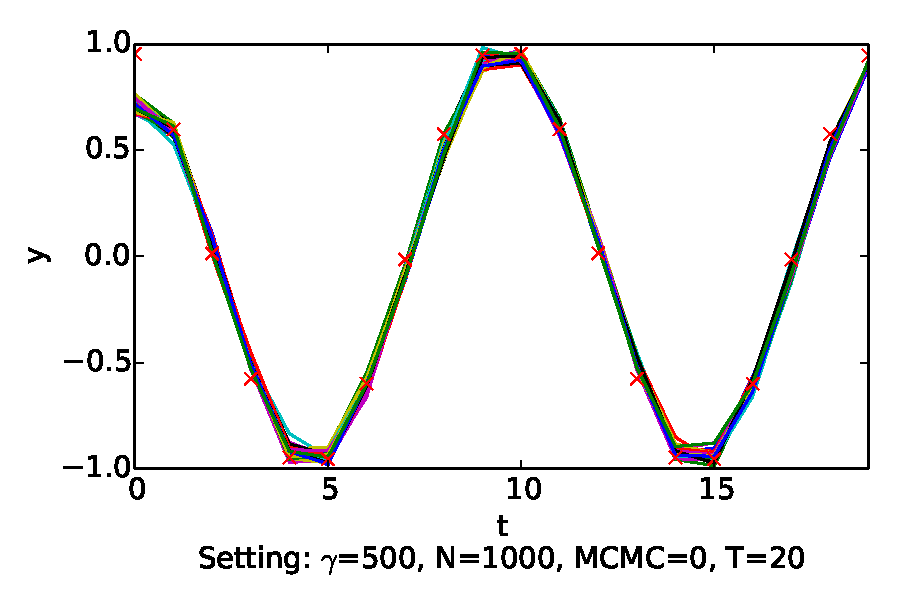
\includegraphics[width=\textwidth]{output_y/output_20_500.pdf}
    \end{minipage}%
    \begin{minipage}{0.5\textwidth}
        \centering
        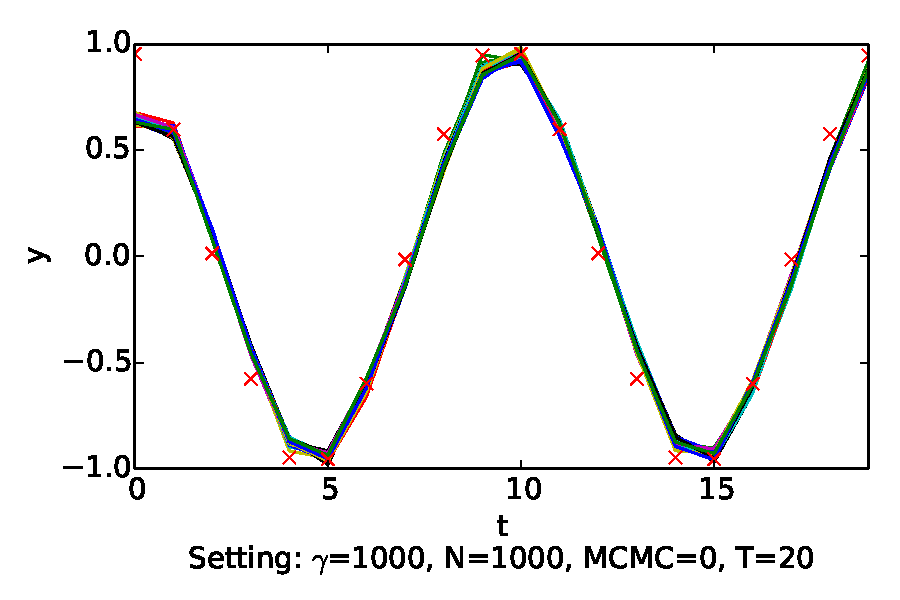
\includegraphics[width=\textwidth]{output_y/output_20_1000.pdf}
    \end{minipage}
    \caption{The means of the recursive likelihood $m_{t \mid t-1}(u^*_{1:T})$ obtained in $30$ independent runs with $T=20$, $N=1000$, various $\gamma$ settings and Resample-Move step disabled are plotted in lines with different colours. The target reference signal $y^{ref}$ is also plotted with a `x' marker.}
    \label{fig:estimatedy}
\end{figure}

\begin{figure}[!thbp]
    \centering
    \begin{minipage}{.5\textwidth}
        \centering
        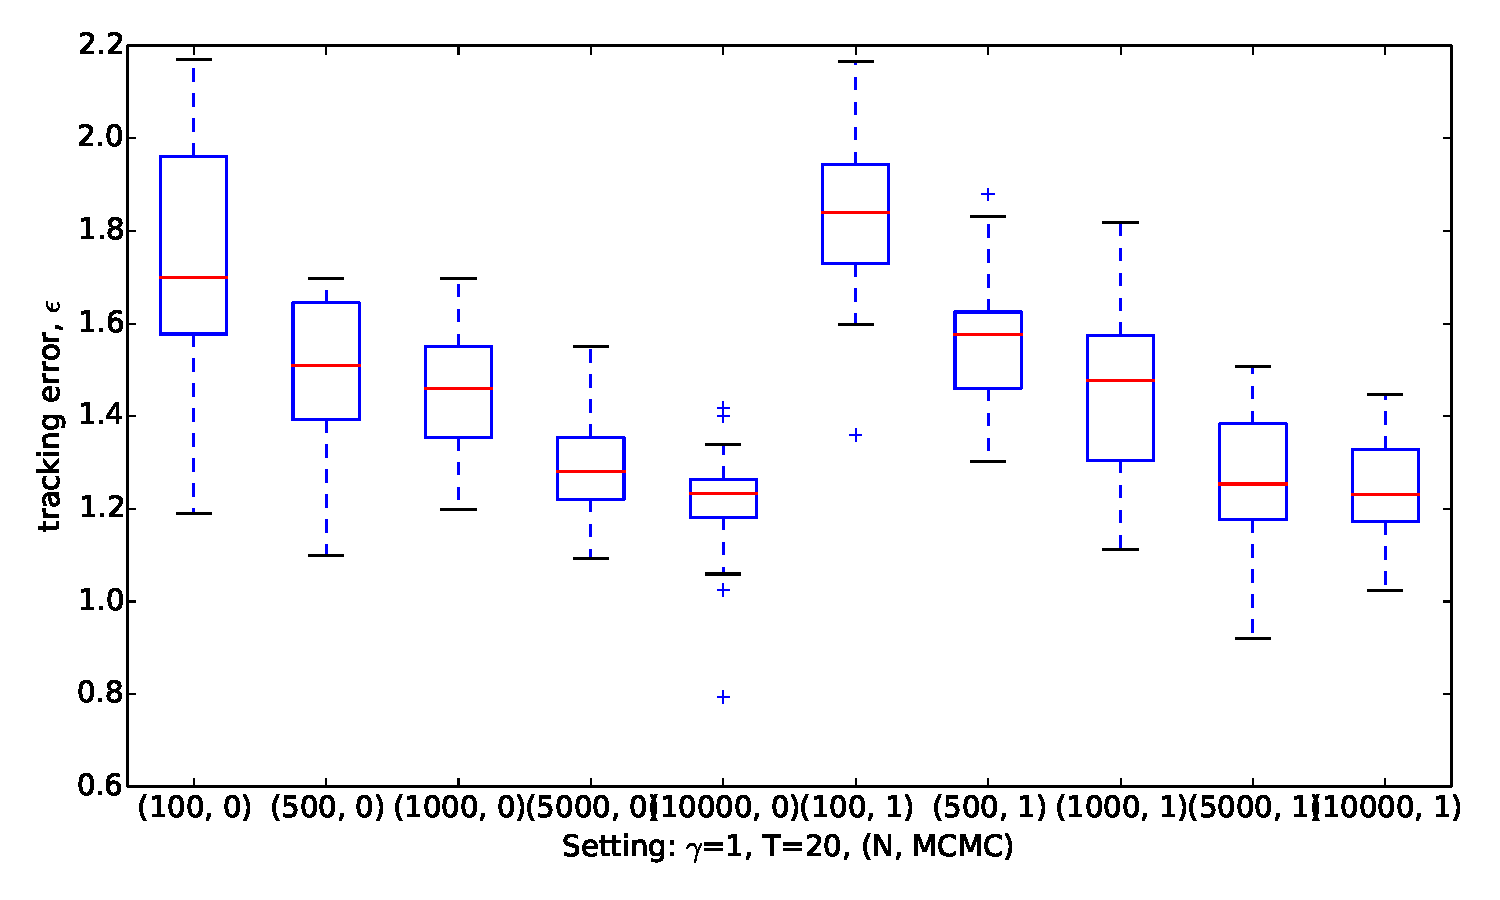
\includegraphics[width=\textwidth]{loglik_t_gs_n_error/T20_gamma1.pdf}
    \end{minipage}%
    \begin{minipage}{0.5\textwidth}
        \centering
        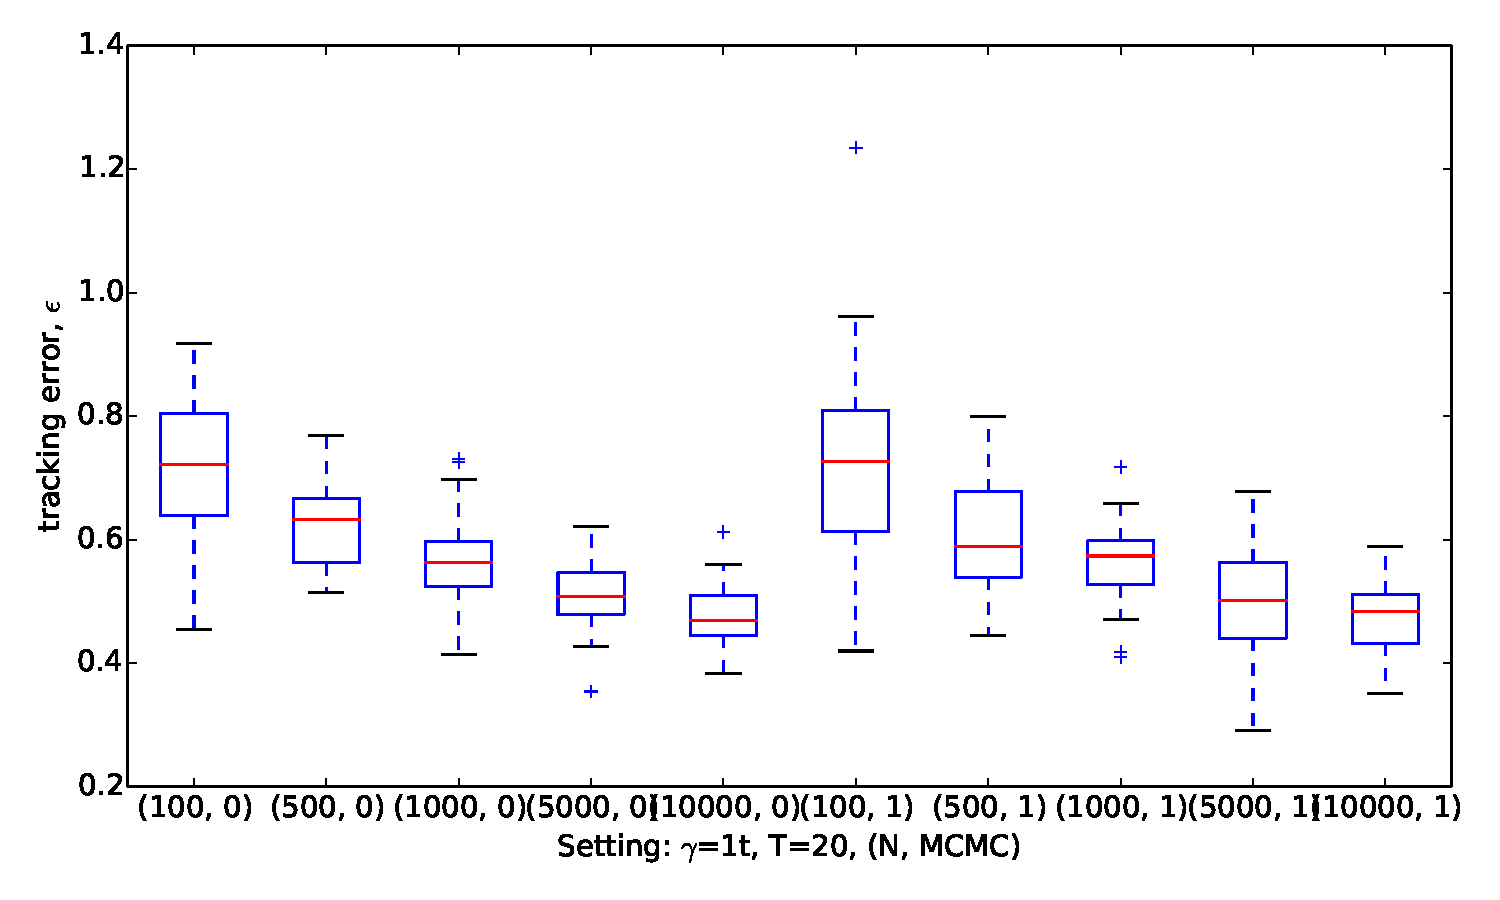
\includegraphics[width=\textwidth]{loglik_t_gs_n_error/T20_gamma1t.pdf}
    \end{minipage}
    \begin{minipage}{0.5\textwidth}
        \centering
        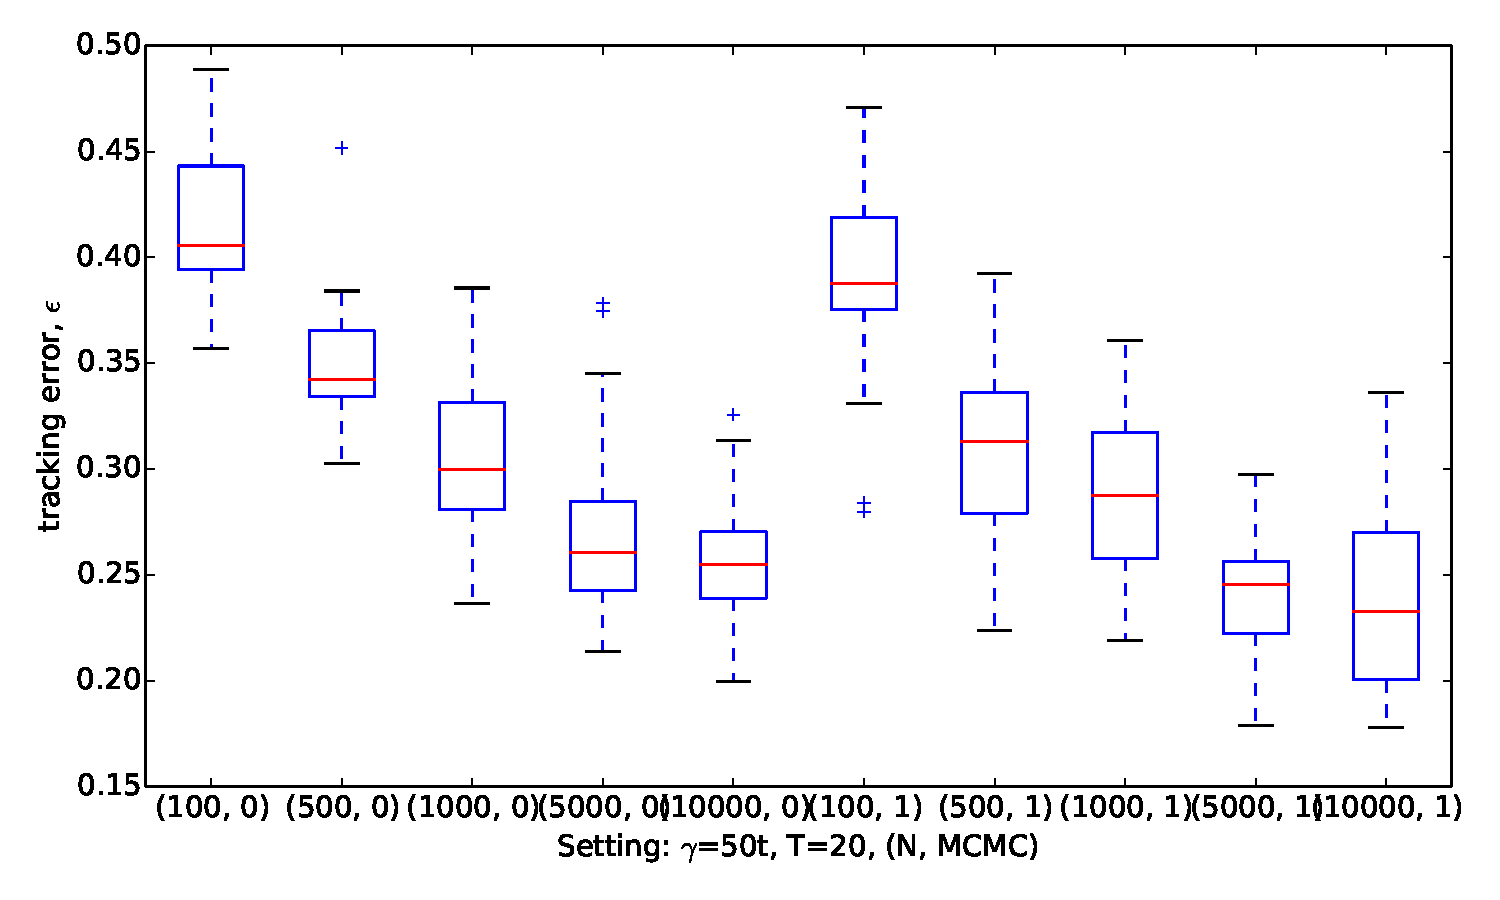
\includegraphics[width=\textwidth]{loglik_t_gs_n_error/T20_gamma50t.pdf}
    \end{minipage}%
    \begin{minipage}{0.5\textwidth}
        \centering
        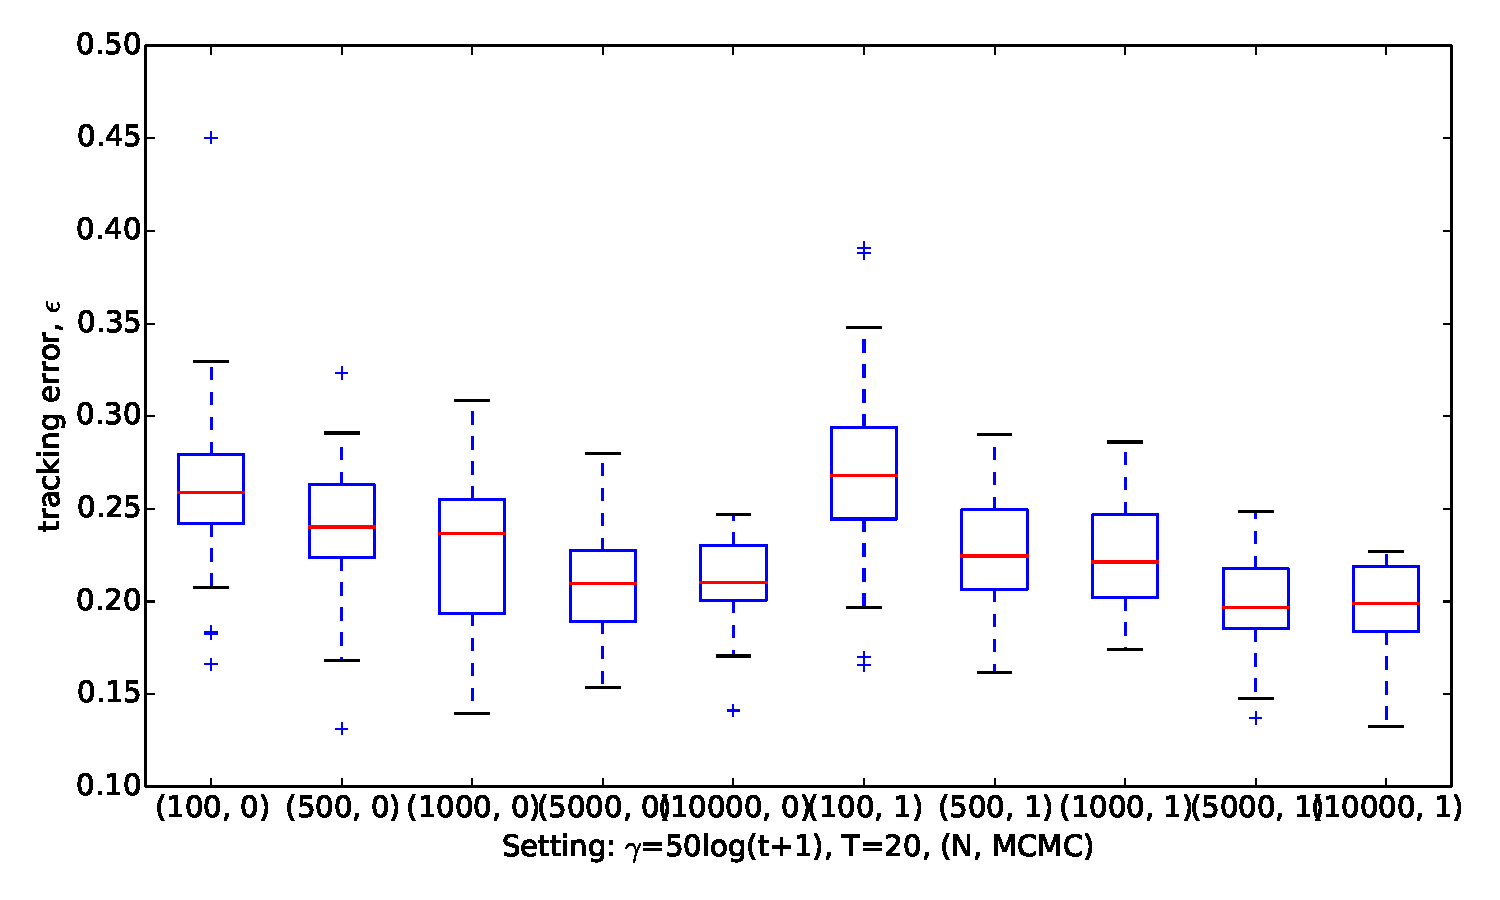
\includegraphics[width=\textwidth]{loglik_t_gs_n_error/T20_gamma50log(t+1).pdf}
    \end{minipage}
    \begin{minipage}{0.5\textwidth}
        \centering
        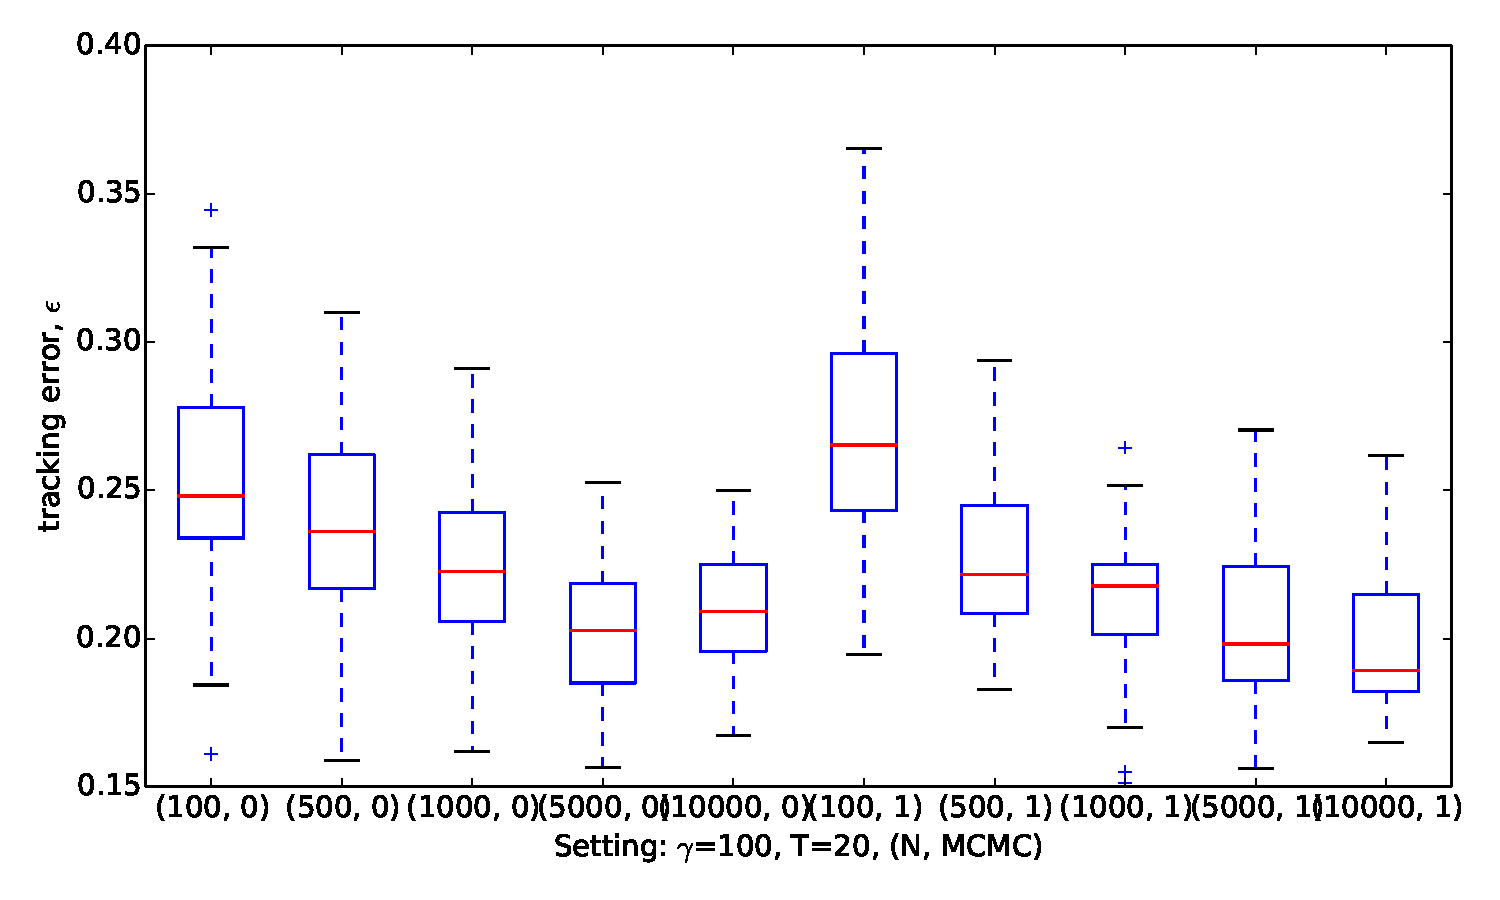
\includegraphics[width=\textwidth]{loglik_t_gs_n_error/T20_gamma100.pdf}
    \end{minipage}%
    \begin{minipage}{0.5\textwidth}
        \centering
        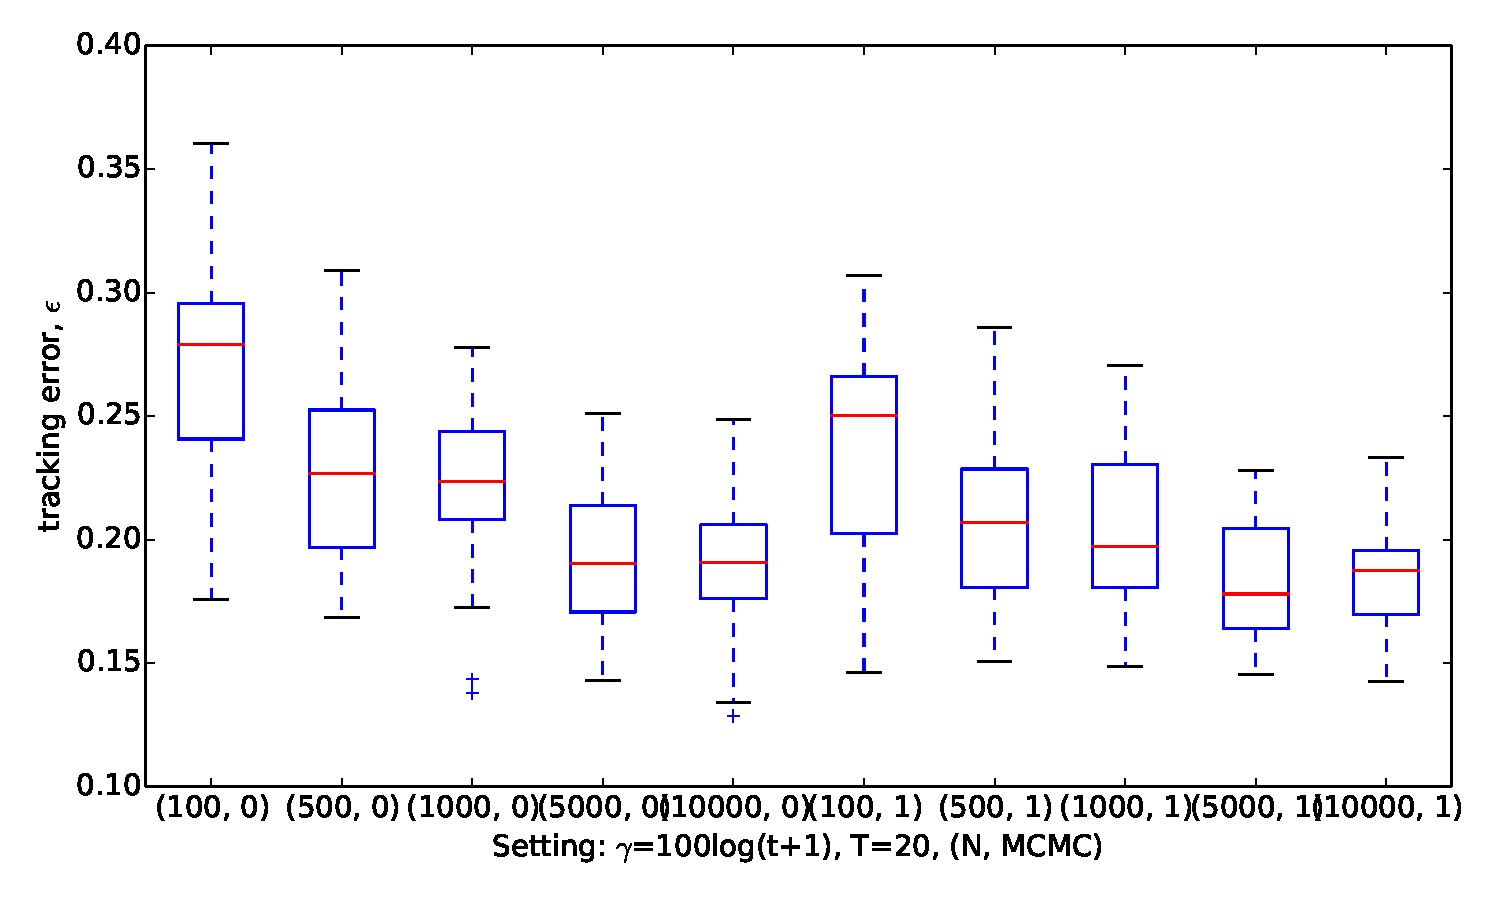
\includegraphics[width=\textwidth]{loglik_t_gs_n_error/T20_gamma100log(t+1).pdf}
    \end{minipage}
    \begin{minipage}{0.5\textwidth}
        \centering
        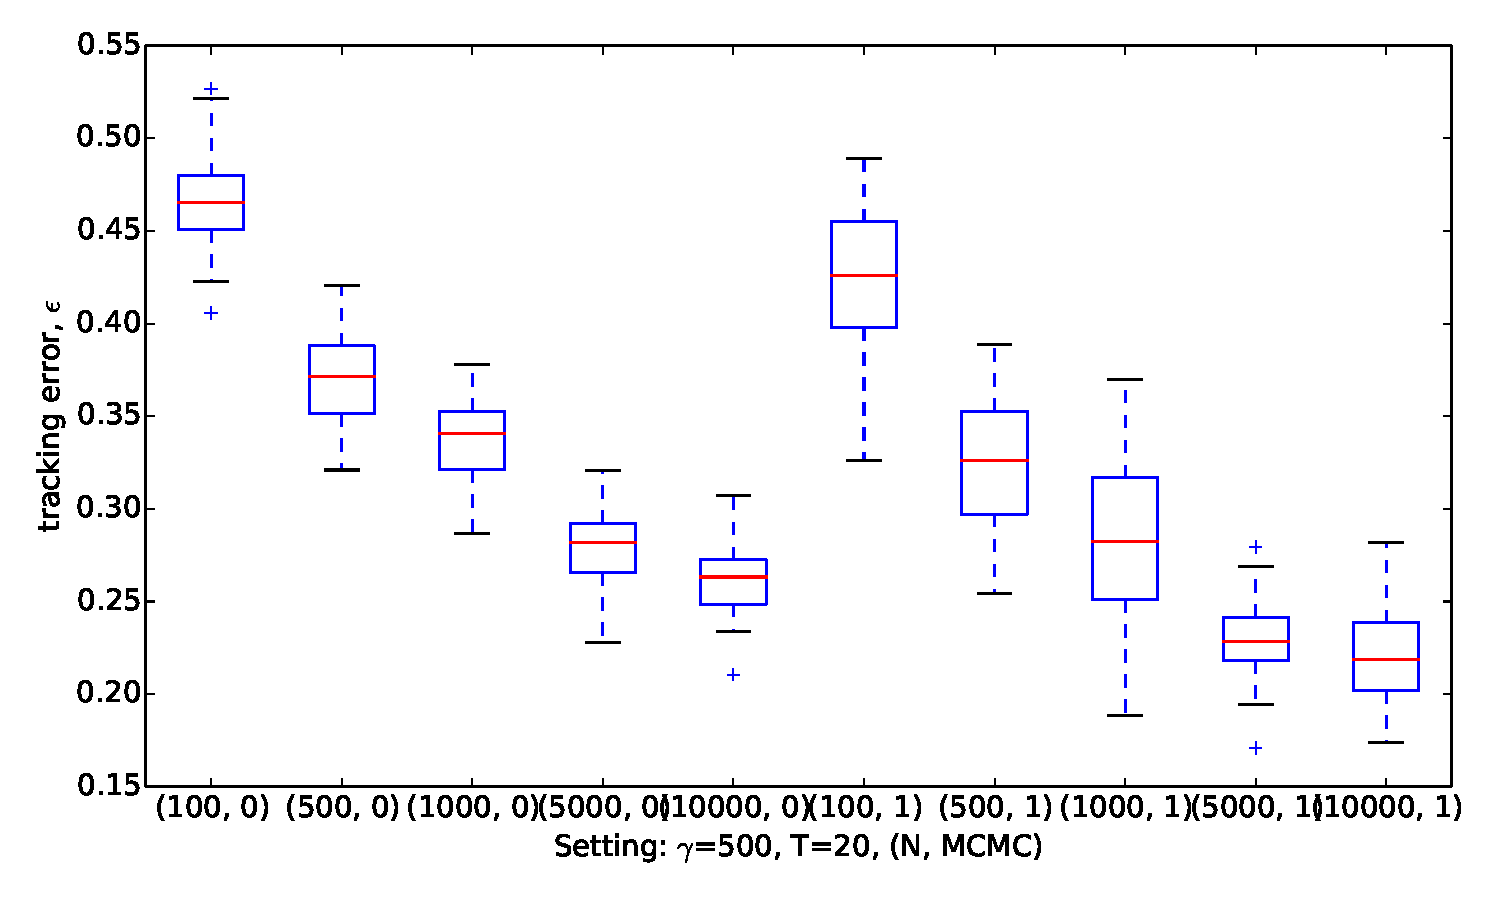
\includegraphics[width=\textwidth]{loglik_t_gs_n_error/T20_gamma500.pdf}
    \end{minipage}%
    \begin{minipage}{0.5\textwidth}
        \centering
        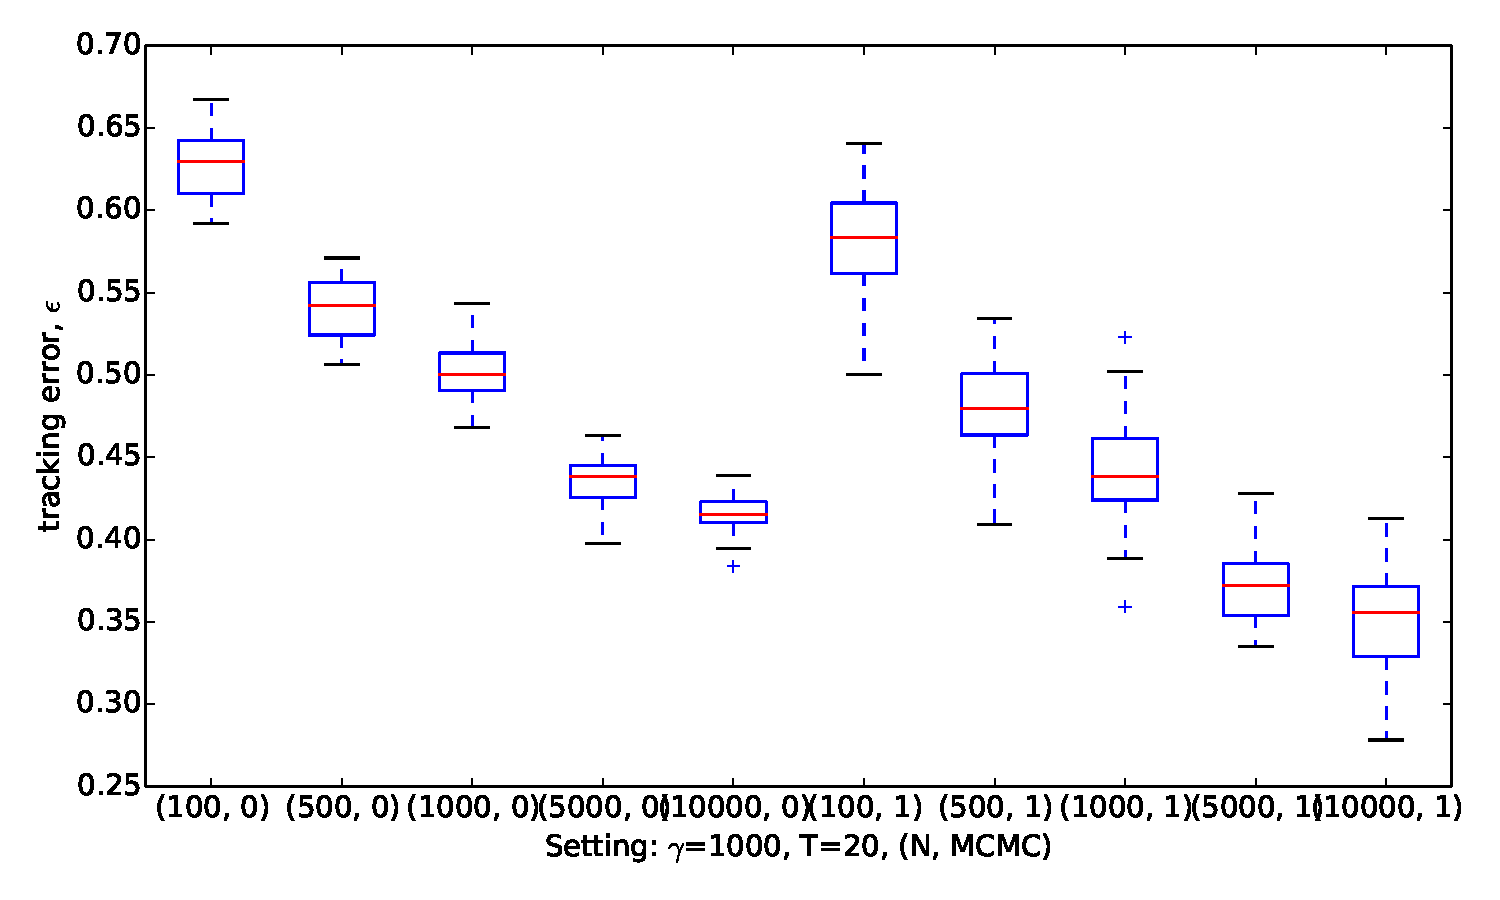
\includegraphics[width=\textwidth]{loglik_t_gs_n_error/T20_gamma1000.pdf}
    \end{minipage}
    \caption{The box-plots of tracking errors of the model using $u^*_{1:T}$ obtained in $30$ independent runs with $T=20$, $N=1000$, various $\gamma$ settings and Resample-Move step disabled.}
    \label{fig:error}
\end{figure}

\section{Conclusions}
In this chapter, we introduce index tracking funds and summarise some causing factors of the tracking error between a fund and its benchmark index. We then present how the portfolio optimisation problem in terms of minimising the tracking error can be formulated as a stochastic control problem. This stochastic control problem can be turned into a path-space parameter estimation problem, in which Rao-Blackwellised SMC can be used to estimate these parameters efficiently. Lastly, we presents a proof-of-concept experiment with a oscillating wave as target reference signal. The results show that the SMC technique proposed is able to track the reference signal well.

\chapter{Tracking the DAX index}
\graphicspath{{Chapter4/figures/}}
\label{cha:dax}
In this chapter, we attempt to use the same SMC technique proposed to a track a real-world financial index. We look at the German's DAX (Deutscher Aktienindex) Index, which consists of 30 German's blue chip stocks listed on Frankfurt Stock Exchange as the constituents from 1st January 2014 up to 30th June 2014. It represents $80\%$ of the aggregated prime standard's market capitalisation. The DAX Index is chosen for various pragmatic reasons. It is one of the major world indices that is tracked by various index funds, it has small number of components and the data is freely accessible\footnote{Actually, we first looked at Dow Jones Industrial Average (DJIA) Index obtained. It was later found some of the data is not publicly available. Having said that, the preliminary findings concur with the findings we have with the DAX Index reported here.}. For further details on the DAX Index methodology, refer \cite{DAX14}.
 
\section{Tracking the DAX4 sub-index}
In the first experiment, we define a simple hypothetical sub-index, DAX4 consists of four stocks from the DAX Index that have the highest weights as of 2nd January 2014, namely Bayer (BAYN), Siemens (SIE), BASF (BAS) and Daimler (DAI). Then, the DAX4 index level is calculated as the simple weighted average of the adjusted close prices obtained from Yahoo Finance as follows:
\begin{equation}
  y^{DAX4} = \sum_{s \in \mathcal{S}} w_s x_s
\end{equation}
where $y^{DAX4}$ is the index level, $\mathcal{S}$ consists of the four stocks and  $w_s$ and $x_s$ are the weight and price of stock $s$ respectively. Here the weights of these four stocks are assigned to be $0.4$, $0.3$, $0.2$ and $0.1$ respectively. The adjusted close price of each stock along with the calculated index level are shown in Figure \ref{fig:adjclose}.
 
\begin{figure}[!thbp]
\centering
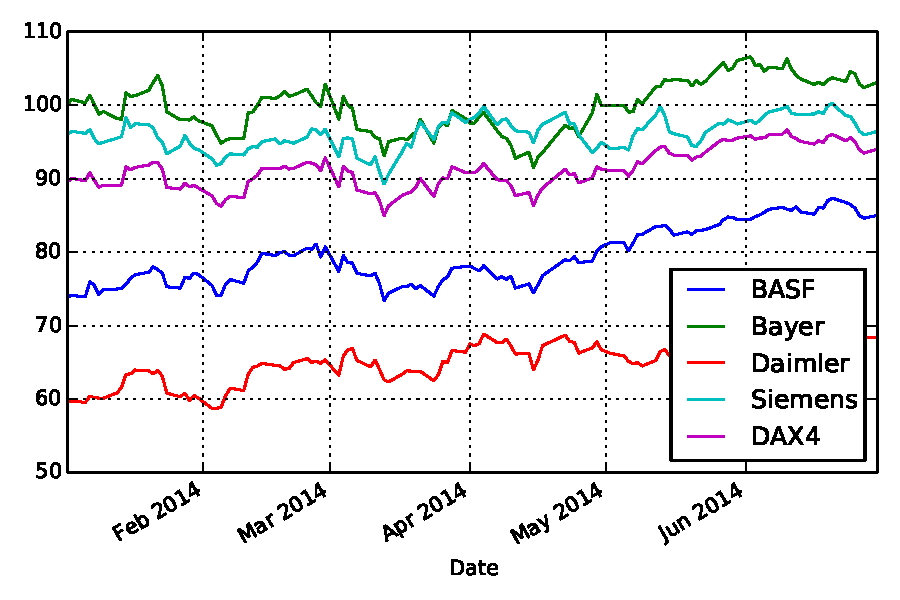
\includegraphics[width=\textwidth]{adjclose}
\caption{The adjusted close price of the 4 stocks and the calculated DAX4 index level, $y^{DAX4}$.}
\label{fig:adjclose}
\end{figure}
 
The portfolio optimisation problem is formulated as such $y^{DAX4}$ is viewed as the target reference level that a portfolio manager attempt to replicate as close as possible by changing the holding position on each component stocks in $\mathcal{S}$, at the same time, minimise the transaction cost incurred in position changes.
 
To solve this problem using the SMC,  the following state space modelling is used:
\begin{align}
  X_t &= X_{t-1} + F_t(U_t) + W_t \\
  Y_t &= U^T_tX_t + 0.01V_t
\end{align}
where $W_t \sim \mathcal{N}(\mu_{t_0}, \Sigma_{t_0})$, $V_t \sim \mathcal{N}(0, I)$, $\{X_t\}_{t \geq 0}$ is a vector of stock price processes modelled as Arithmetic Brownian Motion with drift, $\{U_t\}_{t \geq 0}$ is a vector of control input processes, each component represents the position we have for each stock, $F_t(U_t)$ can be viewed as the market impact on price due to position changes and is set to be $0.0001U_t$ here, $\mu_{t_0}$ and $\Sigma_{t_0}$ are vector of the estimated mean of price changes and the estimated covariance matrix of the price changes and $\{Y_t\}_{t \geq 0}$ is the process represents the index level.

The values of $\mu_t$ and $\Sigma_t$ here are estimated using Exponential Weighted Moving Average (EWMA) approach with the decay rate, $\lambda$, set to $0.94$. For example, $\mu_t$ can be easily calculated in a recursion form as follows:
\begin{equation}
  \mu_t = \lambda \mu_{t-1} + (1-\lambda) r_{t}
\end{equation}
where $r_t$ is the price change at time step $t$. It is obvious from these equations that the EWMA estimate at time $t$ depends on all the preceding estimates at time $s$, where $s < t$. To ensure the quality of EWMA estimate, a 6 months warm up period is used, i.e., the EWMA estimate is calculated starting from 1st July 2013 onwards. The estimates of $\mu_{t_0}$ and $\Sigma_{t_0}$ obtained are as follows:
\begin{equation}
\mu_{t_0} =
\begin{blockarray}{c}
\\
\begin{block}{(c)}
~ 0.03125069 \\
0.20020445 \\
0.08702132 \\
0.18319923 \\
\end{block}
\end{blockarray}
~\Sigma_{t_0} =
\begin{blockarray}{ccccc}
  BAYN & SIE & BAS & DAI & \\
\begin{block}{(cccc)c}
 ~ 0.60011676 & 0.69688309 & 0.44198994 & 0.66709016 ~ & BAYN \\
0.69688309 & 1.34168488 & 0.58394515 & 0.76533660 & SIE \\
0.44198994 & 0.58394515 & 0.48855826 & 0.56500417 & BAS \\
0.66709016 & 0.76533660 & 0.56500417 & 1.13794411 & DAI \\
\end{block}
\end{blockarray}
\end{equation}
 
It is worth here to re-iterate here that this model is just a means to an end to demonstrate the idea. Other sophisticated models, e.g., Geometric Brownian Motion with drift, Jump Diffusion model, etc., are possible, perhaps even better.

Using this model, we can write the reward function as follows:
\begin{equation}
  J(u_{1:T},y^{ref}_{1:T}, x_0) = \E_{x_0}\left[ \exp \left( -\dfrac{1}{2}\displaystyle\sum^T_{t=1}\left(\vert\vert y^{ref}_t - u^T_tx_t \vert\vert^2_{Q_t(u_t)^{-1}}  + \vert\vert u_t - u_{t-1} \vert\vert^2_{L_t}\right) \right ) \right]
\end{equation}
Here, we define $L = 0.1\diag(4,3,2,1)$  and also impose additional constraints on the holding position of each individual component of $U_t$ such that the range is within $[0,0.5]$. The idea behind these choices is to construct a scenario in which the transaction cost involved in changing the holding position on each individual component is different and impose a constraint on the maximum amount on the holding position of each individual component one portfolio can have.

For the sake of simplicity, we will use the SMC algorithm to target $\pi^\gamma$ where $\gamma=100$ and important sampling step, $U_{1,n}$ is sampled uniformly from the range bounded by the constraints mentioned above. The experiment is carried out for $30$ independent runs, each with sample size is fixed to $10000$ and no Resample-Move step is used here.

\subsection{Results and discussion}
As in previous experiment, the estimated optimal control $u^*_{1:T}$ and the mean of the recursive likelihood $m_{t \mid t-1}(u^*_{1:T})$ obtained in one of the independent runs are shown in Figure \ref{fig:dax}.  The output of the model produce using the estimated $\hat{u}^*_{1:T}$ is closely tracking the reference index level, $y^{DAX4}$. The average annualised\footnote{the annualisation factor is set to be $\sqrt{252}$ as the daily return is measured here.} tracking error of $0.023288$ over the $30$ runs. Having said that, the estimated set of control parameter $\hat{u}^*_{1:T}$ which represents the holding position of each stock does not seem very stable.

\begin{figure}[tbp]
\centering
    \begin{minipage}{0.5\textwidth}
        \centering
        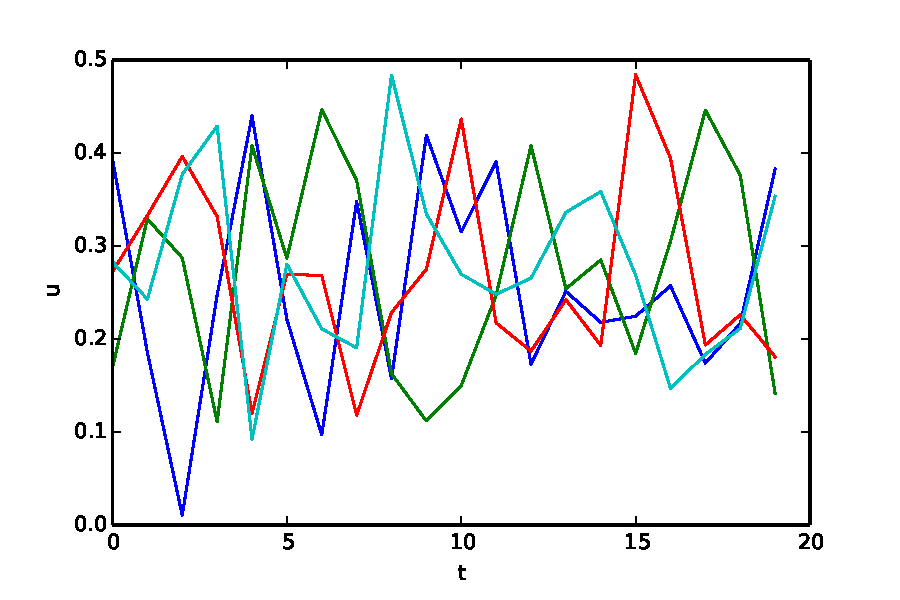
\includegraphics[width=\textwidth]{DAX4Low-u.pdf}
    \end{minipage}%
    \begin{minipage}{0.5\textwidth}
        \centering
        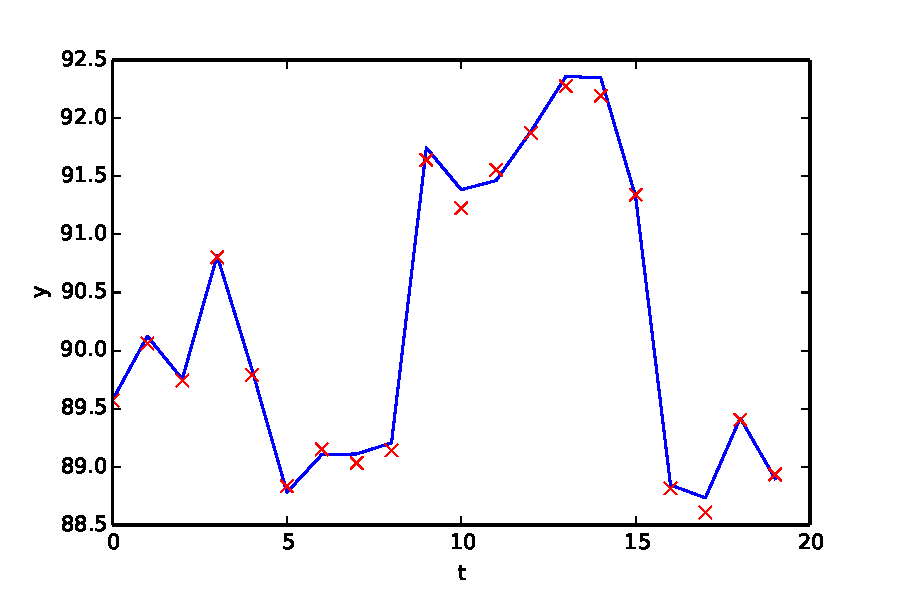
\includegraphics[width=\textwidth]{DAX4Low-y.pdf}
    \end{minipage}
\caption{The estimated optimal control $u^*_{1:T}$ and the mean of the recursive likelihood $m_{t \mid t-1}(u^*_{1:T})$ obtained in one of the independent runs with the $y^{DAX4}$ set to be the target reference using $L = 0.1\diag(4,3,2,1)$.}
\label{fig:dax4}
\end{figure}

To reduce the number of changes in holding positions, the value of $L$ matrix can be scaled up. To demonstrate this, the same experiment is re-run with $L = 5\diag(4,3,2,1)$. The results are shown in Figure \ref{fig:dax42}. The estimated set of control parameters $\hat{u}^*_{!:T}$ produced in this case is much more stable. However, this comes at a price on the tracking error. The average annualised tracking error with this setting is increased to $0.036386$ over the $30$ runs. 

\begin{figure}[htbp]
\centering
    \begin{minipage}{0.5\textwidth}
        \centering
        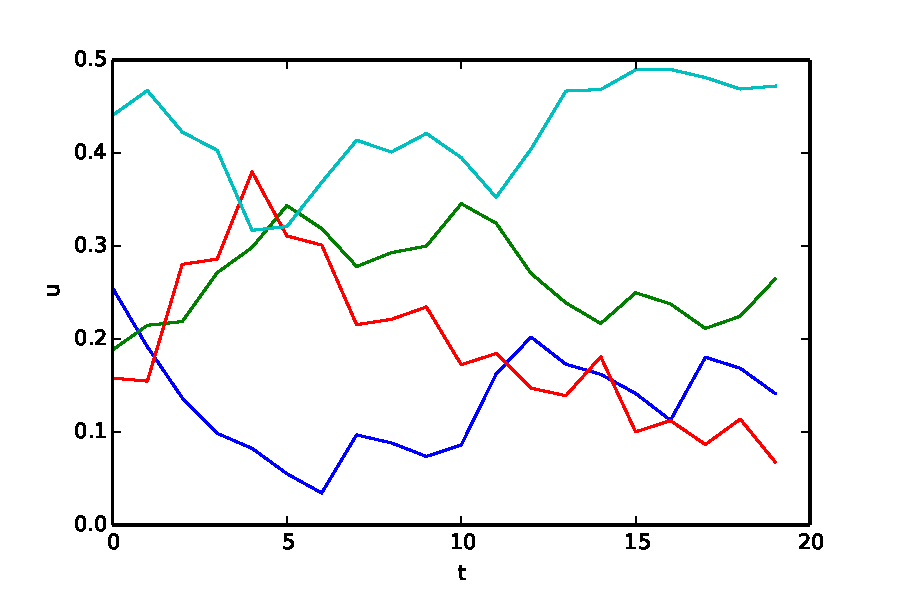
\includegraphics[width=\textwidth]{DAX4High-u.pdf}
    \end{minipage}%
    \begin{minipage}{0.5\textwidth}
        \centering
        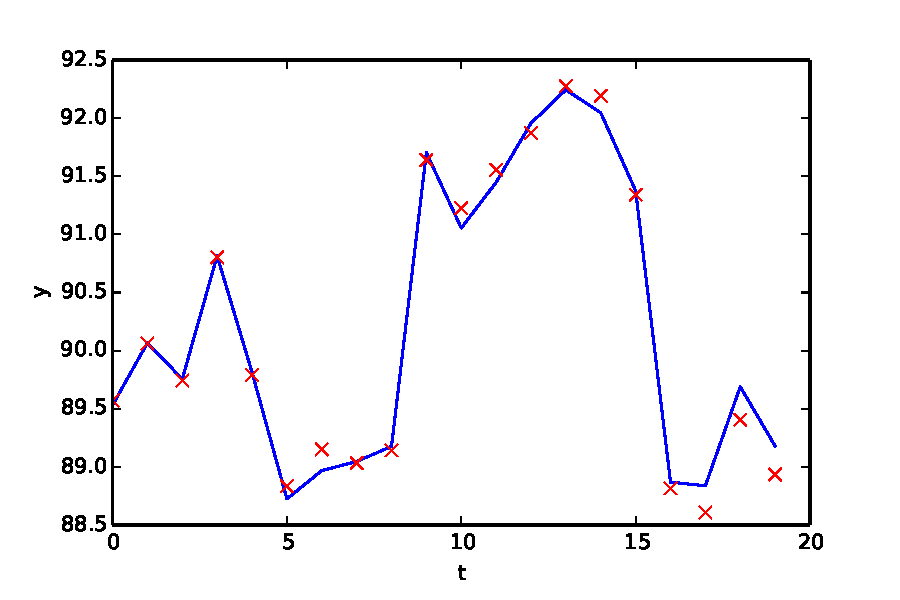
\includegraphics[width=\textwidth]{DAX4High-y.pdf}
    \end{minipage}
\caption{The estimated optimal control $u^*_{1:T}$ and the mean of the recursive likelihood $m_{t \mid t-1}(u^*_{1:T})$ obtained in one of the independent runs with the $y^{DAX4}$ set to be the target reference using $L = 5\diag(4,3,2,1)$.}
\label{fig:dax42}
\end{figure}

\subsection{Tracking the DAX index}
Given the results of the experiment for DAX4 index look promising, we now attempt to track the original DAX index which consists of all $30$ components using a similar model as follows:
\begin{align}
  X_t &= X_{t-1} + F_t(U_t) + W_t \\
  Y_t &= 30U^T_tX_t + 0.01V_t
\end{align}
where $W_t \sim \mathcal{N}(\mu_{t_0}, \Sigma_{t_0})$, $V_t \sim \mathcal{N}(0, I)$, along with the same parameter settings as before except the following:
\begin{enumerate}
\item The target reference $y^{ref}$ is the daily close level of the DAX index level.
\item The number of dimensions for $U_t$ and $X_t$ are now $30$.
\item The $L$ matrix is set to be $5I_{30 \times 30}$, where $I_{n \times n}$ is the $n$ dimensional identity matrix, i.e., the transaction cost of each component is all equal.
\end{enumerate}
The experiment is carried out for $30$ independent runs, each with sample size is fixed to $10000$ and no Resample-Move step is used here.

As mentioned in Section \ref{sec:replication}, instead of tracking the index by fulling replicating all its components, sometimes it can be more efficient not only just in terms of computational, but also in terms of transaction cost and management perspective to track the benchmark index with only a subset of its component stocks.

To do this, only minimal changes are required to apply on the model proposed. We choose to use the top $6$ highest weighted constituents of DAX index by including Allianz SE ($ALV$) and SAP SE ($SAP$), in which they all together constitute more than $50\%$ of the weights for the DAX index level as of 2nd January 2014. Using only these $6$ component stocks and a slight increase on the range of each component of $U_t$ to within $[0,1]$, the experiment is re-run for $30$ times.

\subsubsection{Results and discussion}
As before, the estimated optimal control $u^*_{1:T}$ and the mean of the recursive likelihood $m_{t \mid t-1}(u^*_{1:T})$ obtained in one of the independent runs with the DAX index level set to be the target reference for both the full replication setting and partial replication setting are shown in Figure \ref{fig:dax} and \ref{fig:daxpartial} respectively.

In the full replication setting, the average annualised tracking error over $30$ runs is found to be $0.113118$. However, the computational cost increases significantly in this experiment due to the dimensionality increases in $U$ and $X$. Using the computation cost of the previous $DAX4$ experiment as the baseline, the computational cost for this experiment is $\approx 7.2$ times more per time step.

In the partial replication setting, the average annualised tracking error over $30$ runs is found to be $0.062650$. The estimated optimal control $u^*_{1:T}$ found in this setting is also much stable. This means smaller changes in holding positions and therefore lower transaction costs. In terms of computational cost, the relative computational cost factor in comparison to the baseline is approximately $1.1$. This translates to approximately $6.5\times$ speed-up in comparison to the full replication setting.

\begin{figure}[htbp]
\centering
    \begin{minipage}{0.5\textwidth}
        \centering
        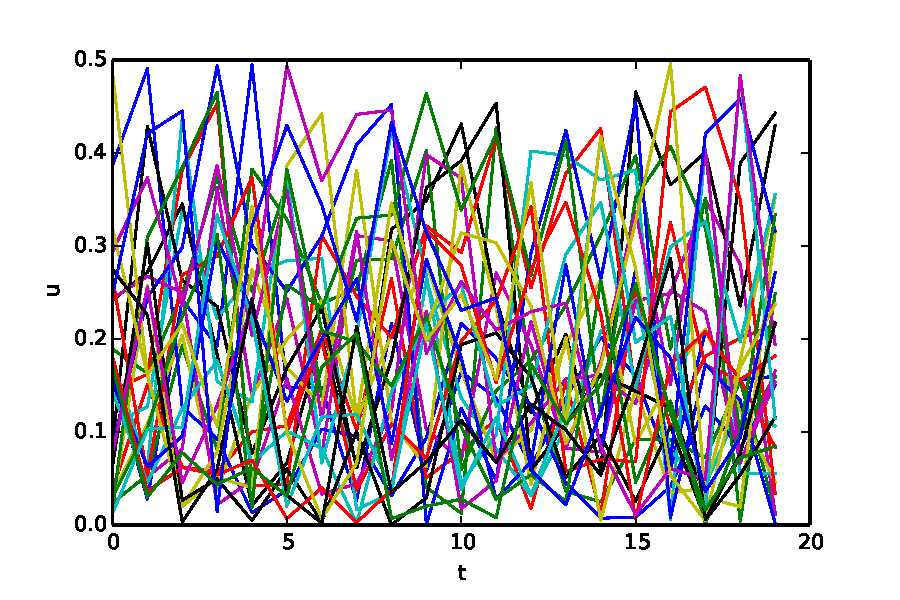
\includegraphics[width=\textwidth]{DAXFull-u.pdf}
    \end{minipage}%
    \begin{minipage}{0.5\textwidth}
        \centering
        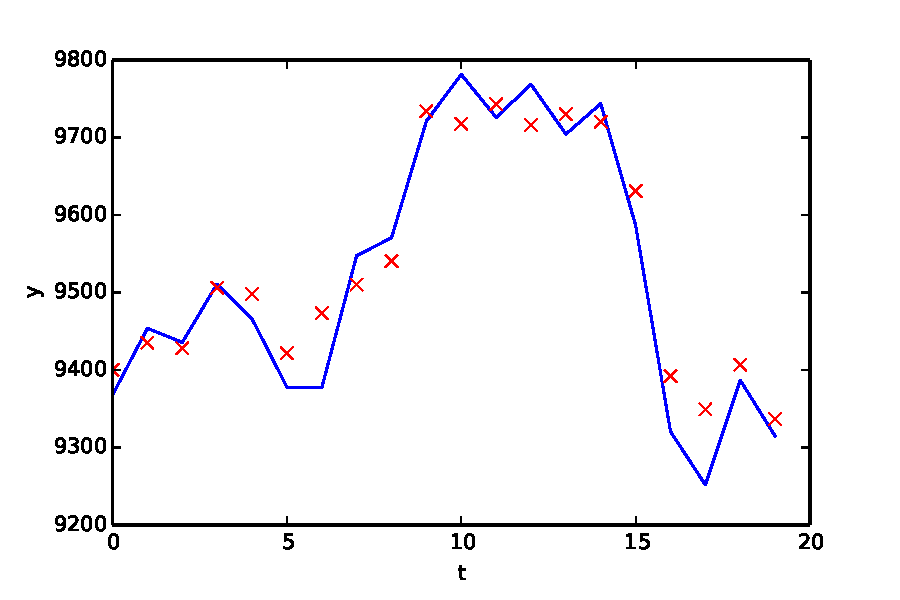
\includegraphics[width=\textwidth]{DAXFull-y.pdf}
    \end{minipage}
\caption{The estimated optimal control $u^*_{1:T}$ and the mean of the recursive likelihood $m_{t \mid t-1}(u^*_{1:T})$ obtained in one of the independent runs with the DAX index level set to be the target reference using all $30$ component stocks.}
\label{fig:dax}
\end{figure}

\begin{figure}[htbp]
\centering
    \begin{minipage}{0.5\textwidth}
        \centering
        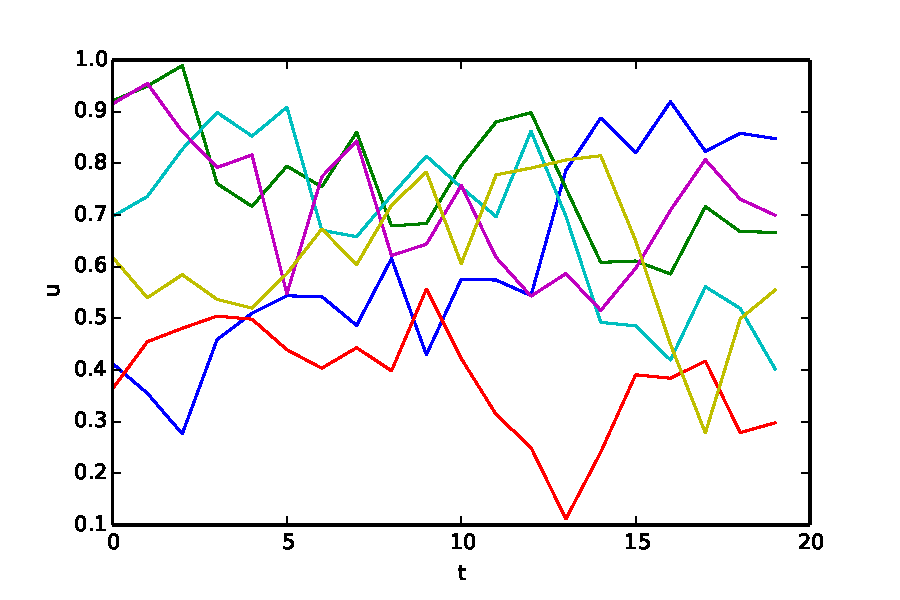
\includegraphics[width=\textwidth]{DAXPartial-u.pdf}
    \end{minipage}%
    \begin{minipage}{0.5\textwidth}
        \centering
        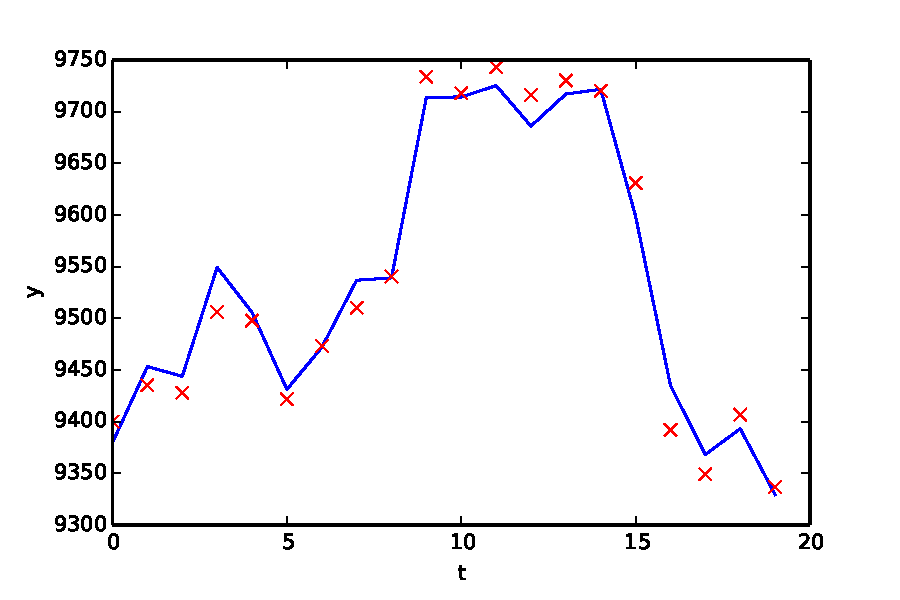
\includegraphics[width=\textwidth]{DAXPartial-y.pdf}
    \end{minipage}
\caption{The estimated optimal control $u^*_{1:T}$ and the mean of the recursive likelihood $m_{t \mid t-1}(u^*_{1:T})$ obtained in one of the independent runs with the DAX index level set to be the target reference using only the top $6$ highest weighted component stocks.}
\label{fig:daxpartial}
\end{figure}

\section{Model Predictive Control (MPC)}
Up to this point, the discussion has been focussed on searching the optimal control parameters for a given time horizon $0:T$ at time step $0$. There are two issues here:
\begin{enumerate}
\item It is assumed that the future target reference signal $y^{ref}_{t^\prime}$, $t^\prime > 0$ is available for optimisation. In this application, but these are in fact not observable as of time step $0$.
\item The optimisation is \emph{only} performed at the beginning of the time horizon, i.e., the problem is treated as an open loop problem. Any new observation of the target reference signal, any of the control used and any of the output produced by the model over the time horizon are not fed back to the system.
\end{enumerate}

To overcome these problems, instead of tracking the true $y^{ref}$, an estimate of $y^{ref}$ is used as the target reference signal whenever the $y^{ref}$ is not (yet) available. A simple estimator of $y^{ref}_{t+s}$ at time step $t$ is defined to be as follows:
\begin{equation}
  \hat{y}^{ref}_{t+s} = y^{ref}_{t} + \beta s
\end{equation}
where $s > 0$, $\beta$ is the EWMA estimate ($\lambda = 0.94$) of the mean of daily changes of $y^{ref}_t$ calculated at time step $t$. This estimator is chosen here for the sake of simplicity. Other estimators are possible. To simplify notation, we will define $\tilde{y}^{ref}_{t^\prime}$ at any time step $t$ to be as follows:
\begin{align}
\tilde{y}^{ref}_{t^\prime} &= y^{ref}_{t^\prime}&\text{if } t^\prime \leq t, \nonumber \\
                                      &= \hat{y}^{ref}_{t^\prime}&\text{otherwise}    
\end{align}

To take into account the any new observable information into account over the time horizon, we employ the Model Predictive Control (MPC) framework. MPC is a receding horizon control algorithm. At time step $t$, the model defined is used to search for the optimal controls, $u^*_{t:t+H}$ for a finite horizon for $t:t+H$, where $H$ is a parameter that defines the size of the short finite horizon. Then, only the first set of controls, i.e., $u^*_{t}$ is applied to the system. At time step $t+1$, the model is updated with new observed information. Using the updated model, the optimisation process is repeated for the same finite horizon, but shifted by $1$ time step. This process is repeated until $t=T$. The MPC framework is summarised in Algorithm \ref{algo:mpc}.  MPC has achieved significant success in many applications, see \cite{RJB09,MJM02} for further details on MPC.

\begin{algorithm}
\caption{Model Predictive Control}\label{algo:mpc}
\begin{algorithmic}[1]
\Function{ModelPredictiveControl}{T,H}
\State Set $t = 1$.
\While{$t \leq T$}
\State Search the optimal $u^*_{t:t+H}$ for the control problem of time horizon $t:t+H$.
\State Apply the first set of the optimal control  $u^*_{t}$ to the problem.
\State Update the model states with any new information.
\State Set $t = t + 1$.
\EndWhile
\EndFunction
\end{algorithmic}
\end{algorithm}

It is straight forward to apply the MPC framework for this problem. At every time step $t$, the SMC optimisation technique proposed can be executed to search for the optimal $u^*_{t:t+H}$, but only the first set of controls, $u^*_t$ is applied the model to produce the output $y$. Using this approach, the reward function that we attempt to optimise at each time step $t$ is as follows:
\begin{equation}
  J(u_{t:t+H},\tilde{y}^{ref}_{t:t+H}, x_t) = \E_{x_0}\left[ \exp \left( -\dfrac{1}{2}\displaystyle\sum^{t+H}_{s=t}\left(\vert\vert \tilde{y}^{ref}_s - u^T_s x_s \vert\vert^2_{Q_s(u_s)^{-1}}  + \vert\vert u_s - u_{s-1} \vert\vert^2_{L_s}\right) \right ) \right]
\label{eq:J2}
\end{equation}
This reward function is different from the previous ones as it does not depend any future information beyond time step $t$.

To demonstrate this idea, we re-run the experiment on the DAX index tracking with partial replication setting using this MPC framework with $H=5$. The experiment is repeated for $30$ times. Figure \ref{fig:mpc2} shows the estimated optimal control $u^*_{1:T}$ and the mean of the recursive likelihood $m_{t \mid t-1}(u^*_{1:T})$ obtained in one of the independent runs. The tracking performance looks very good, with an average annualised tracking error of $0.062364$ over the $30$ runs. The estimated optimal control $u^*_{1:T}$ is also found to be reasonably stable.

In terms of computational cost, the empirical computational cost factor in relative to the baseline is approximately $\approx 5.2$ per run. This makes sense as the complexity of each run here is  $\mathcal{O}(NTH)$ as opposed to $\mathcal{O}(NT)$ in as in the previous case\footnote{We assume here the Resample-Move step is disabled. With Resample-Move step enabled, the complexity of this technique is $\mathcal{O}(NTH^2)$ as opposed to $\mathcal{O}(NT^2)$.}.

\begin{figure}[htbp]
\centering
    \begin{minipage}{0.5\textwidth}
        \centering
        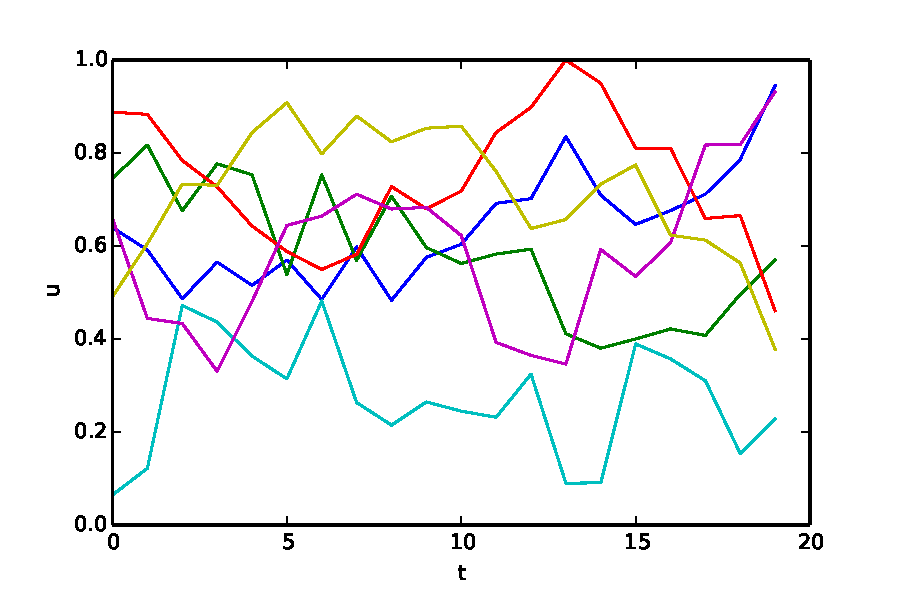
\includegraphics[width=\textwidth]{DAXMPC-u-2}
    \end{minipage}%
    \begin{minipage}{0.5\textwidth}
        \centering
        \includegraphics[width=\textwidth]{DAXMPC-y-2}
    \end{minipage}
\caption{The estimated optimal control $u^*_{1:T}$ and the mean of the recursive likelihood $m_{t \mid t-1}(u^*_{1:T})$ obtained in one of the independent runs with the estimated DAX index level ($\hat{y}^{ref}_{t:t+H}$) set to be the target reference using the MPC framework with $H=5$ and $T=20$.}
\label{fig:mpc2}
\end{figure}

In the last experiment, we attempt to demonstrate the scalability of the technique by considering the same problem, but with an extended time period of $T=125$, i.e., $\approx 6$ months period. Figure \ref{fig:mpc2long} shows the estimated optimal control $u^*_{1:T}$ and the mean of the recursive likelihood $m_{t \mid t-1}(u^*_{1:T})$ obtained in one of the independent runs. Again, the results look promising, with an average annualised tracking error of $0.062364$ over the $30$ runs. 

\begin{figure}[htbp]
\centering
    \begin{minipage}{\textwidth}
        \centering
        \includegraphics[width=\textwidth]{DAXMPC-u-2-long}
    \end{minipage}
    \begin{minipage}{\textwidth}
        \centering
        \includegraphics[width=\textwidth]{DAXMPC-y-2-long}
    \end{minipage}
\caption{The estimated optimal control $u^*_{1:T}$ and the mean of the recursive likelihood $m_{t \mid t-1}(u^*_{1:T})$ obtained in one of the independent runs with the estimated DAX index level ($\hat{y}^{ref}_{t:t+H}$) set to be the target reference using the MPC framework with $H=5$ and $T=125$.}
\label{fig:mpc2long}
\end{figure}

\section{Conclusions}
\label{sec:conclusion5}
This chapter presents several experiments in apply the SMC technique to track a real-world financial index --- the DAX index.  It begins with a simple experiment in which a synthetic sub-index constructed with only $4$ components to proof the concept. It then uses the same technique to demonstrate how the DAX index can be tracked with full replication as well as partial replication. Lastly, it introduces Model Predictive Control (MPC) framework and demonstrates how this technique can be integrated into the MPC framework easily. In all cases, the results show the SMC technique proposed is able to search for the optimal controls that produce an output that tracks the given reference signal well.
